\documentclass[master=mai,english,openright,fleqn]{kulemt}
\setup{title={Classification of human epithelial cell's staining patterns},
  author={Sebastijan Dumancic},
  promotor={Prof.\,dr.\ Hendrik Blockeel},
  assessor={},
  assistant={Antoine Adam}}
  
% The following \setup may be removed entirely if no filing card is wanted%
%\setup{filingcard,
%  translatedtitle=,
%  udc=621.3,
%  shortabstract={Here comes a very short abstract, containing no more than 500
%    words. \LaTeX\ commands can be used here. Blank lines (or the command
%    \texttt{\string\pa r}) are not allowed!
%    \endgraf \lipsum[2]}}
% Uncomment the next line for generating the cover page
%\setup{coverpageonly}
% Uncomment the next \setup to generate only the first pages (e.g., if you
% are a Word user.
%\setup{frontpagesonly}

% Choose the main text font (e.g., Latin Modern)
\setup{font=palatino}

\chapterstyle{veelo}

% If you want to include other LaTeX packages, do it here. 
%\usepackage[utf8]{inputenc}
\usepackage{algpseudocode}
\usepackage{float}
\usepackage{algorithm}
\usepackage{amsmath}
\usepackage{tabulary}
\usepackage{ wasysym }
\usepackage{array}
\usepackage{graphicx}
\usepackage{multirow}
\usepackage{xcolor,colortbl}

\newcommand\MyBox[1]{
  \fbox{\lower0.75cm
    \vbox to 1.7cm{\vfil
      \hbox to 1.7cm{\hfil\parbox{1.0cm}{ #1}\hfil}
      \vfil}%
  }%
}

% Finally the hyperref package is used for pdf files.
% This can be commented out for printed versions.
\usepackage[pdfusetitle,colorlinks,plainpages=false]{hyperref}

%%%%%%%
% The lipsum package is used to generate random text.
% You never need this in a real master thesis text!
\IfFileExists{lipsum.sty}%
 {\usepackage{lipsum}\setlipsumdefault{11-13}}%
 {\newcommand{\lipsum}[1][11-13]{\par And some text: lipsum ##1.\par}}
%%%%%%%

%\includeonly{chap-n}
\begin{document}

\begin{preface}
  %I would like to thank everybody who kept me busy the last year,
  %especially my promotor and my assistants. I would also like to thank the
  %jury for reading the text. My sincere gratitude also goes to my wive and
  %the rest of my family.
  \lipsum[1]
\end{preface}

\tableofcontents*

\begin{abstract}
  The \texttt{abstract} environment contains a more extensive overview of
  the work. But it should be limited to one page.

  \lipsum[1]
\end{abstract}

% A list of figures and tables is optional
%\listoffigures
%\listoftables
% If you only have a few figures and tables you can use the following instead
\listoffiguresandtables
% The list of symbols is also optional.
% This list must be created manually, e.g., as follows:
\chapter{List of Abbreviations and Symbols}
\section*{Abbreviations}
\begin{flushleft}
  \renewcommand{\arraystretch}{1.1}
  \begin{tabularx}{\textwidth}{@{}p{12mm}X@{}}
    LoG   & Laplacian-of-Gaussian \\
    MSE   & Mean Square error \\
    PSNR  & Peak Signal-to-Noise ratio \\
  \end{tabularx}
\end{flushleft}
\section*{Symbols}
\begin{flushleft}
  \renewcommand{\arraystretch}{1.1}
  \begin{tabularx}{\textwidth}{@{}p{12mm}X@{}}
    42    & ``The Answer to the Ultimate Question of Life, the Universe,
            and Everything'' according to \cite{h2g2} \\
    $c$   & Speed of light \\
    $E$   & Energy \\
    $m$   & Mass \\
    $\pi$ & The number pi \\
  \end{tabularx}
\end{flushleft}

% Now comes the main text
\mainmatter



\chapter{Introduction} 

\label{Chapter1} 


%----------------------------------------------------------------------------------------
%	GENERAL INTRODUCTION
%----------------------------------------------------------------------------------------

In the last couple of decades, computers  have found a number of applications in biology and medicine. We may even say they have become an essential tool in revealing the questions of life. A significant role in those problems was played by machine learning, a branch of artificial intelligence concerned with the construction of models capable of learning from data . Probably the most inspiring example comes from the field of bioinformatics where scientists have used the methods from  statistics and artificial intelligence to sequence the human genome for the first time. If that was one of the first results, then, what can we expect from the future? \\

Besides the genomic data which is represented as a sequence of nucleotides, a great amount of  biological data can be aquired by different imaging methods such as microscopy, PET or CT imaging and others. That is were the medical imaging and bioimage analysis fields come from. The field of bioimage analysis studies the biological problems by examining an image, or image sequence of a process of interest, while the medical image analysis is concerned with developing of methods that will help in a medical diagnosis process based on imaging. \\

The above mentioned field of medical image analysis overlaps with a field of computer aided diagnosis (CAD) which collects a broader range of methods used as an assistance to the doctors. An application area of this Thesis would fit the best in that field. This thesis will take a direction in a specific task of assistance to an autoimmune disease diagnosis, with a special emphasis to human interpretable models. During the recent few years, this specific problem has been solved very efficiently. If the problem has been solved, why is this thesis taking another look at it? \\

The goal of the Thesis is to provide a  CAD method capable of making a decision based on a microscopic image of HEp-2 cell in a human intepretable way. To demonstrate the importance of intepretable model in CAD systems, I consider the following scenario.

%----------------------------------
%   MOTIVATIONAL SCENARIO
%----------------------------------

\section{Motivational Scenario}

Imagine a following scenario. \textit{Peter} is a doctor, an immunologist. Being an immunologist, his job is to find out which autoimmune disease a patient has. As that is an extremly hard task, Jules uses  computer assistance - an artifical intelligence program named \textit{Hal}. Hal's role is to confirm Peter's diagnosis, or to provide an additional insight if the decision is hard to make. \\

We are interested in the situation where Peter and Hal have made a conflicted decision. There are two cases representing the insight Hal can provide. Each case reflects Hal's interior structure : a \textbf{black-box} model\footnote{By black-box model we assume a model for which we can only observe it's output, not a decision process} or an \textbf{ interpretable} one. If Hal is the black-box model, it is not much of an assistance, as Hal can't elaborate it's decision. We can only agree we disagree. In this case, Hal is not much of a help. 

On the other hand, if Hal is an interpretable model, it can elaborate it's decision and help Peter. If a wrong decision was made by Hal, Peter can observe it's model parameters, correct the wrong one(s), query again and see if new result supports it's decision. If a wrong decision was made by Peter, Peter can observe Hal's model, find the parameters he might have overseen and correct his diagnosis. 

The example clearly demonstrates one  thing -- the importance of interpretable models for CAD systems. Computers have proven their ability of inferring from a large amount of data, usually outperforming humans, but in specific situations, a good and accurate model is not enough. We also need to interpret results if we are going to use them.

\section{Detecting the autoimmune diseases}

As mentioned already, this Thesis will address the specific topic of autoimmune diseases classification. The human immune system creates antibodies to fight against infections whereas antinuclear antibodies affect healthy tissues. The Antinuclear Autoantibodies test (ANA) is widely used to determine whether the immune system is developing antibodies or not. Indirect immunofluorescence (IIF ) with HEp-2 cells is the recommended method to diagnose the presence of antinuclear autoantibodies in patient serum. \\

IIF method consists of four consecutive steps:
\begin{itemize}
	\item cell segmentation
 	\item intensity level classification
 	\item mitosis detection
 	\item staining pattern classification
\end{itemize}

The final step usually classifies cell images into one of following patterns: homoge
neous, speckled, nucleolar, cytoplasmic, centromere (see figure \ref{fig:CellExamples}). Some variations may be introduced in different datasets due to large number of possible patterns. Those staining patterns further have a clinical associations with a specific autoimmune disease such as Scleroderma, malignant tumor, Lupus nephritis and others. \\

\begin{figure}[htbp]
	\centering
	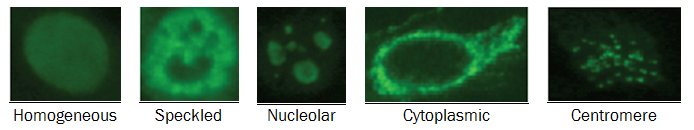
\includegraphics[scale=0.7]{Figures/introduction/cell_examples}
	\rule{35em}{0.5pt}
	\caption[Cell examples]{HEp-2 cell patterns}
	\label{fig:CellExamples}

\end{figure}

Although IIF posses qualities such as high sensitivity and a large number of antigens
that can be detected, it suffers from numerous shortcomings. The most important ones
are liability to subjectivity and time and labour consuming. \\

In order to avoid any kind of subjectivity , there is a great need for standardization and formalization of the mentioned procedure. Addressing this problem calls for CAD techniques which combines methods from machine learning and image analysis.

\section{Problem statement}

The content of the thesis proposes solutions for three major steps in the IFF process.

First of all, in order to find out a cell's pattern, cells should be isolated from an image aquired by IFF. As it is going to be explained (see chapter \ref{Chapter3}), although the problem of cell segmentation has been studied for more than 50 years, segmenting HEp-2 cells still suffers from certain problems, mostly due to different green flourescent protein apsorbtion accross the cells. This thesis proposes a method based on a region growing algorithm that demonstrates an encouraging result for overcoming mentioned problems. 

Once we have isolated the cells, the next step is to determine the fluorescent intensity of an image. The fluorescent intensity level can take three different values, namely \textit{positive}, \textit{intermediate} and \textit{negative}. A negative value means there are no observable cells in an image, while positive marks easily observable cells.  

The final step presents a novel approach to the staining pattern classification. The current state of the art solution solves the problem very succesfully, but acts like  black-box solutions not providing any explanation for the decision. This thesis tends to develop a method based on the human interpretable representation and reasoning. As IF-THEN rules are the most natural way of representing human knowledge,  the thesis will follow a rule mining approach, such as Inductive Logic Programming (ILP).
% Chapter Template

\chapter{Background} 

\label{Chapter2} % Change X to a consecutive number; for referencing this chapter elsewhere, use \ref{ChapterX}

%\lhead{Chapter 2. \emph{Understanding the domain}} % Change X to a consecutive number; this is for the header on each page - perhaps a shortened title

%----------------------------------------------------------------------------------------
%	SECTION 1
%----------------------------------------------------------------------------------------

\section{Understanding the domain}

\subsection{Immune system and antibodies }

The immune system is the central part of the human body responsible for protection against infections. In order to function properly, the immune system has to detect a wide range of threats, and at the same time distinguish them from  healthy tissue. The main weapon the immune system can use are antibodies.   \\

The antibody is a protein complex produced by \textit{B cells} \footnote{ a subgroup of white blood cells, a viral part of the immune system} that initiates an immune response against a target antigen \footnote{Foreign substance that, when introduced into the body, is capable of stimulating an immune response}. Their primal role is to recognize the unique part of the foreign target and  protect the body from infections. The basic organization of the antibody includes two functional domains that, together, resemble the letter Y (Figure \ref{fig:AntibodyIllustration}, left). The \textit{Fab}  part makes up the arms of the Y, and it contains the antigen-binding site - the region responsible for antigen binding. The \textit{Fc} part comprises the tail of the Y and effects other cells, proteins and antibodies.  \\

This unique structure allows detection of antigens, in direct or indirect manner. By direct detection we assume detection using a single fluorophore-labeled antibody, and by indirect detection we assume detection through binding of a fluorophore-labeled secondary antibody raised against the Fc part of an unlabeled primary antibody (as illustrated in Figure \ref{fig:AntibodyIllustration}, right). This system is versatile and cost-effective because few labeled antibodies are required to detect many possible primary antibodies. \\


\begin{figure}[htbp]
	\centering
	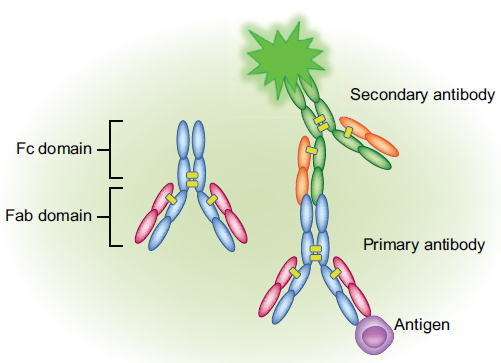
\includegraphics[scale=0.5]{Figures/Domain/antibodies}
	\rule{35em}{0.5pt}
	\caption[Illustration of antibody structure]{Illustration of antibody structure (from \cite{OdellCook2013})}
	\label{fig:AntibodyIllustration}

\end{figure}

The immune system can sometimes suffer from different disorders. A disorder of special importance to this Thesis is  \textit{autoimmunity}. Autoimmunity results in the disability of the immune system to recognize an organism's healthy tissue, and therefore attacks normal tissues as if they were foreign organisms. In the case of autoimmunity, antibodies are called antinuclear antibodies. We can observe those antibodies by using indirect immunofluorescence. \\

\subsection{Indirect Immunofluorescence}

As it was already mentioned, the indirect detection is the main focus of the thesis. Indirect immunofluorescence is a diagnostic methodology based on image analysis that reveals the presence of autoimmune diseases by searching for antibodies in the patient serum. Indirect immunofluorescence is a two-step technique, in which a primary, unlabeled antibody binds to the target, after which a fluorophore-labeled\footnote{fluorophore-labeling is a method to color the antibodies so they can be observed under the microscope} second antibody is used to detect the first antibody (figure \ref{fig:AntibodyIllustration}, right). Indirect immunofluorscence is more sensitive than a direct one because more than one secondary antibody can bind to each primary antibody, which amplifies the fluorescence signal. \\

As a result of its effectiveness,there has been a growing demand for diagnostic tests for systemic autoimmune diseases. Unfortunately,  IIF still remains a subjective method that depends too heavily on the experience and expertise of the physician. The main reasons causing the problems are:
\begin{itemize}
	\item the lack of quantitative information supplied to physicians
	\item varieties of reading systems and optics
	\item the photo-bleaching effect caused by a light source irradiating the cells over a short period of time
	\item the low reproducibility of the diagnostic protocol.
\end{itemize}

\subsection{Putting it all together}

The focus of this thesis is on the Antinuclear antibodies  test (ANA), which plays the main role in the serological\footnote{Further explanation} diagnosis of autoimmune disease. ANAs are directed against a variety of antigens and can be detected in patient serum through laboratory tests. IIF uses the human epithelial (HEp-2) substrate, which bonds with serum antibodies forming a molecular complex. This complex then reacts with human immunoglobulin \footnote{Immunoglobulin is a specific type of antibody created by plasma cells} and becomes visible under a fluorescence microscope which reveals the antigen-antibody reaction. \\

The procedure of ANA starts with  fluorescence intensity classification, a segmentation step is not a part of ANA procedure. The Center for Disease Control and Prevention in Atlanta,USA have published  guidelines \cite{nakamura1996quality} for scoring the intensity. The score ranges from 0 to 4+ as follows:
\begin{itemize}
	\item 4+ : brilliant green (maximal fluorescence)
	\item 3+ : less brilliant green fluorescence
	\item 2+ : defined pattern but diminished fluorescence
	\item 1+ : very subdued fluorescence
	\item 0 : negative.
\end{itemize}

Although the guidelines provide  very detailed instructions, in \cite{Rigon2007} Rigon et al. analyzed the variability between a set of physician's fluorescence intensity  classifications. Their work has shown a big variance of classifications made by physicians on the same dataset, so they suggested to classify the fluorescence intensity into three classes, namely negative, intermediate and positive. This work follows the protocol. \\

The final step consists of staining pattern recognition. As shown in figure \ref{fig:CellExamples}, there are several patterns that may be observed. \cite{FoggiaBenchmarks2013} and \cite{Perner02miningknowledge} provide a description of all staining patterns which is a valuable input taking into consideration a human interpretable perspective of this step. A summary is presented here:
\begin{itemize}

	\item \textbf{Centromere}: characterized by several discrete speckles ( $\sim$ 40 - 60) distributed throughout the interphase\footnote{The interphase is the nonmitotic phase of the cell cycle in which the cell spends the majority of its time and performs the majority of its purposes} nuclei and characteristically found in the condensed nuclear chromatin during mitosis as a bar of closely associated speckles.
	
	\item \textbf{Nucleolar}: characterized by clustered large granules in
the nucleoli of interphase cells which tend towards homogeneity, with less than six granules per cell.

	\item \textbf{Homogeneous}: characterized by a diffuse staining of the interphase nuclei and staining of the chromatin of mitotic cells.
	
	\item \textbf{Fine Speckled}: characterized by a fine granular nuclear staining of the interphase cell nuclei.
	
	\item \textbf{Coarse Speckled}: characterized by a coarse granular nuclear staining of the interphase cell nuclei.
	
	\item \textbf{Cytoplasmatic}: characterized by a highly irregular shape and large granule in the nucleoli

\end{itemize}


%------------------------------------------%
%                                          %
%           MACHINE LEARNING               %
%                                          %
%------------------------------------------%

\section{Machine learning}
% Chapter Template

\chapter{Literature overview} 

\label{Chapter3} % Change X to a consecutive number; for referencing this chapter elsewhere, use \ref{ChapterX}

%\lhead{Chapter 3. \emph{Literature overview}} % Change X to a consecutive number; this is for the header on each page - perhaps a shortened title

%----------------------------------------------------------------------------------------
%	SEGMENTATION
%----------------------------------------------------------------------------------------

\section{Cell segmentation}

Several studies have been proposed to classify autoantibody fluorescence patterns by using an automatic thresholding method, i.e.  Otsu's method, to segment the cells. The  thresholding method can choose the threshold to minimize the intraclass variance of the black and white pixels automatically. Due to the variety of ANA patterns,  Otsu's algorithm always failed to segment cells of speckled and nucleolar patterns, such as cases of a very blury image of low intensity. Figure \ref{fig:BadSegment} shows the over-segmentation results by using Otsu's algorithm. Additional challenge for the segmentation here is to separate overlapping cells which are quite common in the process.

\begin{figure}[htbp]
	\centering
	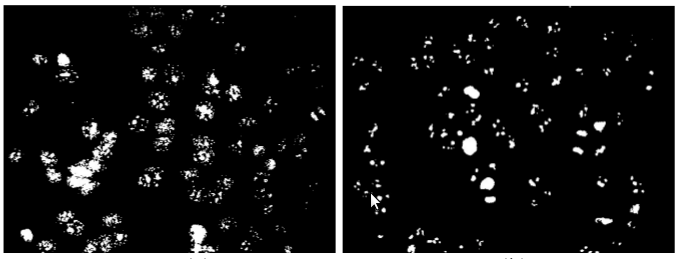
\includegraphics[scale=0.4]{Figures/introduction/badsegmentation}
	\rule{35em}{0.5pt}
	\caption[Bad segmentation example]{Segmentation results of the Otsu method (from \cite{Huang2008})}
	\label{fig:BadSegment}

\end{figure}


In \cite{Huang2008}, Huang et all. present an adaptive edged-based segmentation method for automatically detecting outlines of fluorescence cells in IIF images. Their approach is based on specific properties of the images regarding the pattern class. They have divided the images in two groups : sparse region and mass region cells. The mass region cells are those ones which have a \textit{compact} appearance, that look like a smooth object, while the sparse region cells are those ones for which we can detect multiple object in a cell. The approach trains a classifier to classify each image in the groups and applies different segmentation procedure for each group. In the case of the mass region cells, the cells are segmented using Otsu segmentation method, while in the case of the sparse region cell segmentation is performed by an edge detection. Their approach resulted in better segmentation results, but approximately 10\% of the cells remained undetected. \\

In \cite{HuangWatershed}, same authors further improve their method by incorporating watershed segmentation. The second approach also includes segmentation in two stages, depending on defined criteria. After a segmentation step performed by the watershed, the approach merges parts located relatively close and eliminates parts not large enough to represent a cell. If the retrieved number of regions doesn't safisfy the defined criteria, the segmentation step is performed again with different parameter settings determinated by Otsu's thresholding. \\

All forementioned approaches report similar shortcomings : approximately 10\% of cells remained undetected and the inability to separate overlapping cells.  The focus of the segmentation part of the Thesis will be on overcoming those problems. \\



%-----------------------------------------------------------------------------------------
%   INTENSITY LEVEL CLASSIFICATION
%-----------------------------------------------------------------------------------------

\section{Intesity level classification}

The following step, the intensity level classification, hasn't attracted a lot of scientific research, but has demonstrated remarkable results so far. \\

In \cite{SodaIntensity2006},  authors propose a system based on  \textit{Multi-Layer Perceptrons} and a \textit{Radial Basis Network} for the intensity classification step. That system, which makes use of features inspired from medical practice, shows error rates  up to 1\%, but it uses a reject option and it does not cast a result in about 50\% of cases. In \cite{SodaIntensity2009} the authors further refine their system. They train three experts, one specialized for each class, with a different set of features. They threat the classifiers similar to the \textit{one-vs-all} approach, so the final decision is made by a classifier most certain in it's decision. The authors report a success rate of 92,6\% accuracy. \\


%-----------------------------------------------------------------------------------------
%   STAINING PATTERN CLASSIFICATION
%-----------------------------------------------------------------------------------------

\section{Staining pattern classification}

As this problem was emphasized on the \textit{International Conference on Pattern Recognition 2012} as a contest, this step has been well researched and several very successful methods have been proposed. In \cite{FoggiaBenchmarks2013}, Foggia et al. provides a detailed overview of the methods submitted for the contest. The three most successful ones are presented here.  \\

In \cite{Kuan2012}, Kuan presents a method based on four texture descriptors: a rotation invariant form of local binary patterns (LBP) with multi-scale analysis,discrete cosine transformation, the mean values and standard variances of 2-D Gabor wavelets, and some global appearance based statistical features. A multiclass SVM was trained on each class of the four feature sets. The SVMs are then integrated in one classifier by using the AdaBoost.M1 algorithm. \\

In \cite{Nosaka2012}, Nosaka presents a similar approach on an extension of LBP, namely CoALBP \cite{Nosaka2011}. The advantage of this method is that the method can observe not only locals LBP, but also the spatial relations among adjacent LBP. The classifier is a linear SVM trained on an extended dataset including the rotated patterns of the original images. \\

Xianfeng et al. proposed a system based on MR8 method \cite{Varma2005} to extract statistical intensity features. The method calculates filter responses locally on the image, and then trains a global texton dictionary using $K$-means clustering. In that way, each image is represented by the frequency histogram of textons. The decision is made by a $k$-NN classifier. \\

Although there are many more papers in existance covering this problem, they are not presented here due to different, and not so rigorous, evaluation. Most of the early work was done on private datasets not available to public, which makes them not comparable to the new research results. Other papers with  a more recent date do not follow the evaluation procedure, so it is very hard to compare their efficiency with those ones in the overview. \\

More recently, a new overview of the method was presented by Agrawal et al. in \cite{Agrawal2013}. The committee of \textit{ICPR'13} has released a new, much bigger dataset for the same problem. The authors experimented with the most commonly used features in the previous contest - statistical features, histograms of oriented gradients, shape and size descriptors and texture descriptors. They have chosen the most typical representatives of classifiers, namely Naive Bayes, k-NN, SVM and Random forest. The SVM with Law's textural representation significantly  outperformed other classifiers and feature representations.



% Chapter Template

\chapter{Cell segmentation} % Main chapter title

\label{Chapter4} % Change X to a consecutive number; for referencing this chapter elsewhere, use \ref{ChapterX}


%----------------------------------------------------------------------------------------
%	INTRODUCTION
%----------------------------------------------------------------------------------------

Finding the cells in images is the first and crucial step in the procedure. The problems encountered in the cell segmentation are discussed in Chapter \ref{Chapter3}. All of the problems occur due to coloring procedure that is time dependent, so cells expose different intensity levels over an image. Because of that, part of cells remains undetected and overlapping. The challenge here is to find a method that can overcome different illumination of objects. Proposed solution deals with mentioned problems in separate steps. \\


The proposed solution is based on an observation that, although cells exhibit different properties across image due to different illumination levels, the background is uniform over a whole image and exhibit constant properties. Following the observations, as summarized in algorithm X, the method first segments the background to find locations of the cells and then uses second segmentation step to refine the borders of cells. \\



%----------------------------------------%
%                                        %
%         REGION GROWING                 %
%                                        %
%----------------------------------------%


\section{Background segmentation}

The first step of background segmentation is intended to overcome the problem of undetected cells. A desirable property of segmentation algorithm for this task is the capability of capturing the global properties of the background region across an image. One such algorithm is \textit{Region growing}. Region growing is a simple method that extends a region based on a similarity in intensity levels - the intensity of each candidate pixel is compared with a mean intensity of a current region. If a difference is less than a given threshold, the pixel is added to region. The algorithm is summarized in algorithm \ref{alg:RegGrow}. \\

\begin{algorithm}
\caption{Region Growing }
  \label{alg:RegGrow}
\begin{algorithmic}[1]
 \Function{RegionGrowing}{\textit{starting point, criteria}}
 \State $\mathtt{candidates} \gets \{ \mathtt{neighborhood}(\mathtt{starting \ point}) \}$
 \State $\mathtt{region} \gets \{ \mathtt{starting \ point} \}$
 \State $\mathtt{current point} \gets \mathtt{starting \ point}$
 \While{no new candidates}
 	\For{each candidate of current point}
 		\If{candidate satisfies criteria}
 			\State add it to region
 			\State update parameters of region
 		\EndIf 
 	\EndFor
 	\State $\mathtt{current point} \gets \mathtt{next \ point \ from \ border}$
 \EndWhile
 \EndFunction
\end{algorithmic}
\end{algorithm}

The bottleneck of the method is the evaluation of candidate pixels. If target regions are big, as in this case, the method could be very slow. To overcome this bottle neck, the method is extended with a pre-filling step in which a part of an image is assigned to belong to the background by default. As it can be noticed from images, the majority of image is a dark background which can be observed in an image histogram as the highest peak. To speed up the segmentation, every pixel with intensity lower or equal to the highest peak is automatically assigned to background.   \\

The critical issue here is the estimation of a threshold for comparison. It is a parameter that depends on a distribution of intensities over an image. In a sense, this parameter models a variance in intensity of the background region. Motivated by a variance fitting, the proposed solution is based on an assumption that an image histogram should consist of two regions - one modeling the background and a second one modeling cells, as illustrated in image \ref{img:Histogram}. The goal now is to find those two regions in a histogram. One way to accomplish that is to approximate a histogram with a mixture of Gaussian functions. This approach is taken here.  

\begin{figure}
	\begin{center}
		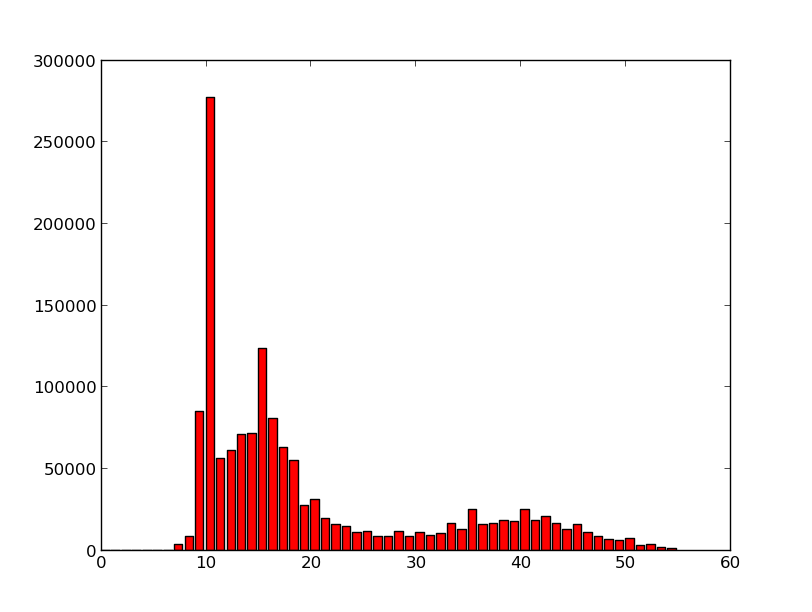
\includegraphics[scale=0.4]{Figures/segmentation/raw_histogram}
		\caption{Example of an image histogram}
		\label{img:Histogram}
	\end{center}
\end{figure}

%-----------------------------------------------------------------------------------------
%     GAUSSIAN MIXTURE MODELS
%-----------------------------------------------------------------------------------------

\subsection{Gaussian mixture model} 

Mixture density is a linear combination of \textit{K} probabilistic density functions:

\begin{equation}
	p(\mathbf{x}) = \sum_{k=1}^{K}\pi_k p(\mathbf{x} | \theta_k)
	\label{eq:GMM}
\end{equation}
	 
where $p(\mathbf{x} | \theta_k)$ represents mixture components with their parameters $\theta_k$. In out case, those mixture components are Gaussian functions $\mathcal{N}(\mu_k, \Sigma_k)$. Parameters $\pi_k$ are mixture coefficients that satisfy $1 \leq \pi_k \leq 1$ and $\sum_{k=1}^{K} \pi_k = 1$. As they satisfy given criteria, those coefficient can be treated as prior probability of a component $k$. Equation \ref{eq:GMM} can be then rewritten as :

\begin{equation}
	p(\mathbf{x}) = \sum_{k=1}^{K} P(\mathcal{G}_k) p(\mathbf{x} | \mathcal{G}_k),
\end{equation}

where $P(\mathcal{G}) = \pi_k$ and $ p(\mathbf{x} | \theta_k) =  p(\mathbf{x} | \mathcal{G}_k)$. Out task is to determine the parameters

\begin{equation}
	 \theta = \{ P(\mathcal{G}_k), \theta_k \}_{k=1}^K,
\end{equation}


or more precisely for the Gaussian function

\begin{equation}
	 \theta = \{ P(\mathcal{G}_k), \mu_k, \Sigma_k \}_{k=1}^K.
\end{equation}


An efficient algorithm to determine those values is the Expectation Maximization algorithm.



%------------------------------------------------------------------------------------------
%     EM ALGORITHM
%------------------------------------------------------------------------------------------

\subsection{Expectation Maximization Algorithm}

The goal of the Expectation Maximization algorithm is to find parameters $\theta$ that maximize the log-likelihood 

\begin{equation}
	\mathcal{L}(\theta | \mathcal{D}) = \mathtt{ln}\prod_{i=1}^{N}p(\mathbf{x}^{(i)}) = \mathtt{ln}\prod_{i=1}^{N}\sum_{k=1}^{K}p(\mathbf{x}^{(i)} | \theta_k) = \sum_{i=1}^{N}\mathtt{ln}\sum_{k=1}^{K}p(\mathbf{x}^{(i)} | \theta_k).
\end{equation}

Unfortunately, there is no closed-form solution for this formulation. Model $p( \mathbf{X} | \boldsymbol \theta)$ is extended with latent variable $\mathbf{Z}$ which determines to which cluster belongs every $x_i$. The density function is now described with $p(\mathbf{X}, \mathbf{Z} | \boldsymbol \theta)$. Marginal density $p(\mathbf{X} | \theta)$, which is density we want to estimate, can always be reconstructed from joint probability by marginalization :

$$ p(\mathbf{X} | \theta) = \sum_{\mathbf{Z}}p(\mathbb{X}, \mathbf{Z} | \boldsymbol \theta). $$

Log-likelihood we try to maximize is now

\begin{equation}
	\mathtt{ln}\mathcal{L}(\boldsymbol \theta | \mathbf{X}) = \mathtt{ln}p(\mathbf{X} | \boldsymbol \theta) = \mathtt{ln}\sum_{\mathbf{Z}}p(\mathbf{X}, \mathbf{Z} | \boldsymbol \theta).
\end{equation}

As values of the latent variable $\mathbf{Z}$ are not yet known, we still can't work with log-likelihood directly. Instead, we will work with the expectation of the log-likelihood $\mathbb{E}[ \mathtt{ln} \mathcal{L}(\boldsymbol \theta | \mathbf{X}, \mathbf{Z}) ]$. The main idea behind the EM-algorithm is to iteratively adjust parameters $\boldsymbol \theta$ to maximize the expectation. \\

The maximization of  $\mathbb{E}[ \mathtt{ln} \mathcal{L}(\boldsymbol \theta | \mathbf{X}, \mathbf{Z}) ]$ is now done by switching between two steps -- E-step and M-step. E-step (\textit{expectation step}) calculates the expectation of the log-likelihood with respect to current values of the parameters  $ \boldsymbol\theta^{(t)}$. That expectation $\mathcal{Q}( \boldsymbol \theta | \boldsymbol \theta^{(t)})$ we can calculate as

\begin{equation} \label{eq1}
\begin{split}
  \mathcal{Q}(\boldsymbol \theta | \boldsymbol \theta^{(t)}) &= \mathbb{E}_{\mathbf{Z} | \mathbf{X}, \boldsymbol \theta^{(t)}}[ \mathtt{ln} \mathcal{L}(\theta | \mathbf{X}, \mathbf{Z}) ] \\
     &= \mathbb{E}_{\mathbf{Z} | \mathbf{X}, \theta^{(t)}}[ \mathtt{ln} p(\mathbf{X}, \mathbf{Z} | \theta) ] \\
      &= \sum_{\mathbf{Z}}P(\mathbf{Z}| \mathbf{X}, \boldsymbol \theta^{(t)})\mathtt{ln} p(\mathbf{X}, \mathbf{Z} | \boldsymbol \theta). \\
\end{split}
\end{equation}

The expectation is now expressed on variable $\mathbf{Z}$ with fixed values of $\mathbf{X}$ and $\theta$. Probability $P(\mathbf{Z}| \mathbf{X}, \boldsymbol \theta^{(t)})$ is the a posteriori  probability of the latent variable $\mathbf{Z}$ with fixed parameters which can be evaluated using Bayes rule. \\

Only thing left is to optimize the parameters $\boldsymbol \theta$. M-step (\textit{maximization step}) chooses new parameters $\boldsymbol \theta^{(t+1)}$ by maximizing the expression

\begin{equation}
	\boldsymbol \theta^{(t+1)} = \arg \max_{\theta}\mathcal{Q}(\boldsymbol \theta | \boldsymbol \theta^{(t)}).
\end{equation}
EM-algorithm is briefly summarized in Algorithm \ref{alg:EM}. Starting with the initial parameters $\boldsymbol \theta^{(0)}$, it iteratively switches between E and M step until converged. The convergence is guaranteed as algorithm maximizes the expectation in every iteration. On the other hand, found solution might not be the global optimum. \\

\begin{algorithm}
\label{alg:EM}
\caption{Expectation-maximization algorithm}

\begin{algorithmic}[1]
 	\Function{EM}{}
 		\State Initialize parameters $\boldsymbol \theta^{(0)}$
 		\State \textit{t} $\leftarrow$ 0
 		\Repeat
 			\State \textbf{E-step:} calculate $P(\mathbf{Z} | \mathbf{X}, \boldsymbol \theta^{(t)})$
 			\State \textbf{M-step:} $\boldsymbol \theta^{(t+1)} \leftarrow \arg\max_{\theta}\mathcal{Q}(\boldsymbol \theta | \boldsymbol \theta^{(t)})$ 
 			 \Statex \quad \quad \quad \quad where $\mathcal{Q}(\boldsymbol \theta | \boldsymbol \theta^{(t)}) = \sum_{\mathbf{Z}}P(\mathbf{Z}|\mathbf{X}, \boldsymbol \theta^{(t)}) \mathtt{ln}p(\mathbf{X}, \mathbf{Z}| \boldsymbol \theta)$
 			\State $t \leftarrow t+1$
 		\Until{converged}
 	\EndFunction
\end{algorithmic}
\end{algorithm}


%---------------------------------------------%
%                                             %
%               EM for GMM                    %
%                                             %
%---------------------------------------------%



\subsection{EM algorithm for mixture models}

The EM-algorithm for mixture models works as follows. Let $\mathbf{z} = (z_1, \ldots, z_K)$ be a latent variable vector indicating a cluster to which an example belong to. $z_k = 1$ if an example belongs to a cluster $\mathcal{G}_k$, $z_k=0$ otherwise. Each cluster is assigned with a prior probability 
$$ P(z_k = 1) = \pi_k, $$
such that $\sum_k\pi_k=1$. Distribution over a latent variable $\mathbf{z}$  hence can be expressed as 

\begin{equation}
	P(\mathbf{z}) = \prod_{k=1}^K\pi_k^{z_k}.
\end{equation}

To evaluate the probability $p(\mathbf{x}, \mathbf{z} | \boldsymbol \theta)$ we are still missing the factor $p(\mathbf{x}| \mathbf{z}, \boldsymbol \theta)$. It can be expressed as 

\begin{equation}
	p(\mathbf{x}| \mathbf{z}, \boldsymbol \theta) = \prod_{k=1}^{K}p(\mathbf{x}| \boldsymbol \theta_k)^{z_k}.
\end{equation}

Joint probability $p(\mathbf{x}, \mathbf{z} | \boldsymbol \theta)$ can now be expressed as 
\begin{equation}
	p(\mathbf{x}, \mathbf{z} | \boldsymbol \theta) = P(\mathbf{z})p(\mathbf{x}| \mathbf{z}, \boldsymbol \theta) = \prod_{k=1}^K\pi_{k}^{z_k}\prod_{k=1}^Kp(\mathbf{x}| \boldsymbol \theta_k)^{z_k}.
	\label{EMM:joint}
\end{equation}

Using the obtained model \ref{EMM:joint}, the log-likelihood $\mathtt{ln}\mathcal{L}(\boldsymbol \theta | \mathcal{D}, \mathcal{Z})$ can be expressed. Take $\mathcal{D} = \{ \mathbf{x}^(i) \}_{i=1}^N$ as a set of examples and $\mathcal{Z} = \{ \mathbf{z}^{(i)} \}_{i=1}^N$ as a set of latent variables describing the relationship between examples and model. Log-likelihood of the model \ref{EMM:joint} is 

\begin{equation}
\begin{split}
	\mathtt{ln}\mathcal{L}(\boldsymbol \theta | \mathcal{D}, \mathcal{Z}) &= \mathtt{ln}\prod_{i=1}^N p(\mathbf{x}^{(i)}, \mathbf{z}^{(i)} | \boldsymbol \theta) = \mathtt{ln}\prod_{i=1}^N\prod_{k=1}^K \pi_k^{z_k^{(i)}}p(\mathbf{x}^{(i)} | \boldsymbol \theta_k)^{z_k^{(i)}} \\
	&= \sum_{i=1}^N \sum_{k=1}^Kz_k^{(i)} \left ( \mathtt{ln}\pi_k + \mathtt{ln}p(\mathbf{x}^{(i)} | \boldsymbol \theta_k)  \right ).
\end{split}
\end{equation}

\subsubsection{E-step}

In E-step of the algorithm we need to calculate the expectation $\mathcal{Q}(\boldsymbol \theta | \boldsymbol \theta^{(t)})$:

\begin{equation}
	\begin{split}
		\mathcal{Q}(\boldsymbol \theta | \boldsymbol \theta^{(t)}) &= \mathbb{E}_{\mathit{Z} | \mathcal{D}, \theta^{(t)}}[ \mathtt{ln}\mathcal{L}(\boldsymbol \theta | \mathcal{D}, \mathcal{Z}) ] \\
		&= \mathbb{E}_{\mathit{Z} | \mathcal{D}, \theta^{(t)}} \left [ \sum_{i=1}^N \sum_{k=1}^K z_k^{(i)} \left ( \mathtt{ln}\pi_k + \mathtt{ln}p(\mathbf{x}^{(i)} | \boldsymbol \theta_k)  \right ) \right ] \\
		&= \sum_{i=1}^N \sum_{k=1}^K \mathbb{E} \left [ z_k^{(i)} | \mathcal{D}, \boldsymbol \theta^{(i)} \right ] \left ( \mathtt{ln}\pi_k + \mathtt{ln}p(\mathbf{x}^{(i)} | \boldsymbol \theta_k)  \right ).
	\end{split}
\end{equation}

As $z_k^{i}$ is a Bernoulli variable (as only one component of $\mathbf{z}^{(i)}$ can be 1) which depends only on one example from $\mathcal{D}$, $\mathbf{x}^{(i)}$, it holds

\begin{equation}
	\mathbb{E} \left [ z_k^{(i)} | \mathcal{D}, \boldsymbol \theta^{(t)}  \right ] = \mathbb{E} \left [ z_k^{(i)} | \mathbf{x}^{(i)}, \boldsymbol \theta^{(t)}  \right ] = P(z_k^{(i)} = 1 | \mathbf{x}^{(i)}, \boldsymbol \theta^{(i)}).
\end{equation}

The expectation of the latent variable equals to its \textit{a posteriori } probability and it can be evaluated by applying the Bayes rule:

\begin{equation}
	\begin{split}
		P(z_k^{(i)} = 1 | \mathbf{x}^{(i)}, \boldsymbol \theta^{(i)}) &= \frac{p(\mathbf{x}^{(i)}| z_k^{(i)} = 1, \boldsymbol \theta^{(t)})P(z_k^{(i)}=1)}{ \sum_{j=1}^{K} p(\mathbf{x}^{(i)}| z_j^{(i)} = 1, \boldsymbol \theta^{(t)})P(z_j^{(i)}=1) } \\
		&= \frac{p(\mathbf{x}^{(i)}| z_k^{(i)} = 1, \boldsymbol \theta^{(t)})\pi_k^t}{\sum_{j=1}^{K} p(\mathbf{x}^{(i)}| z_j^{(i)} = 1, \boldsymbol \theta^{(t)})\pi_j^t} \equiv h_k^{(i)}.
	\end{split}
\end{equation}

Hence, the expectation of the log-likelihood equals

\begin{equation}
	\mathcal{Q}(\boldsymbol \theta | \boldsymbol \theta^{(t)}) = \sum_{i=1}^N \sum_{k=1}^K h_k^{(i)}\mathtt{ln}\pi_k + \sum_{i=1}^N \sum_{k=1}^K h_k^{(i)}\mathtt{ln}p(\mathbf{x}^{(i)} | \boldsymbol \theta_k).
	\label{eq:LogLik}
\end{equation}

\subsubsection{M-step}

M-step maximizes the log-likelihood obtained in \ref{eq:LogLik}. The solution is found analytically by solving $\nabla_{\boldsymbol \theta} \mathcal{Q}(\boldsymbol \theta | \boldsymbol \theta^{(t)})$. To obtain the mixture components, $\pi_k^{(t+1)}$, the equation is $\nabla_{\pi_k}\mathcal{Q}(\boldsymbol \theta | \boldsymbol \theta^{(t)})$. As the second term in \ref{eq:LogLik} does not depend on $\pi_k$, so it can be ignored. Starting from 

\begin{equation}
	\nabla_{\pi_k} \left ( \sum_{i=1}^N \sum_{k=1}^K h_k^{(i)} \mathtt{ln}\pi_k + \lambda \left ( \sum_k\pi_k - 1 \right )  \right ) = 0,
\end{equation}

where \textit{Langrange multiplier} is used to satisfy the condition $\sum_{k=1}^{K} = 1$, it can be easily obtained 

\begin{equation}
	\pi_k^{(t+1)} = \frac{1}{N} \sum_{i=1}^N h_k^{(i)}.
\end{equation}

To find parameters of each component, $\boldsymbol \theta_k^{(i)}$, the equation $\nabla_{\theta_k} \mathcal{Q}(\boldsymbol \theta | \boldsymbol \theta^{(t)}) = 0$ has to be solved. Now first term in the equation \ref{eq:LogLik} does not depend on $\boldsymbol \theta_k$ so it can be ignored 

\begin{equation}
	\nabla_{\theta_k} \sum_{i=1}^N \sum_{k=1}^K h_k^{(i)}\mathtt{ln}p(\mathbf{x}^{(i)} | \boldsymbol \theta_k).
\end{equation}

Substituting $p(\mathbf{x}^{(i)} | \boldsymbol \theta_k)$ with a multidimensional Gaussian distribution and deriving with regards to $\boldsymbol \mu_k$ and $\boldsymbol \sigma_k^2$ new parameters are calculated

\begin{equation}
	\boldsymbol \mu_k^{(t+1)} = \frac{\sum_ih_k^{(i)}x^{(i)}}{\sum_ih_k^{(i)}} 
\end{equation}

\begin{equation}
	(\boldsymbol \sigma^2)_k^{(i)} = \frac{\sum_ih_k^{(i)}(x^{(i)} - \mu_k^{(t+1)})(x^{(i)} - \mu_k^{(t+1)})^T}{{\sum_ih_k^{(i)}}}.
\end{equation}

%---------------------------------------------%
%                                             %
%                 THRESHOLD                   %
%                                             %
%---------------------------------------------%

\subsection{Threshold estimation}

Once histogram has been approximated with two Gaussian functions, obtained functions are used to find a threshold. Such approximation is illustrated in figure \ref{img:Approx}. A Gaussian with a lower mean is assumed to model the background. By examining its variance, the threshold is estimated. The threshold is now defined as a distance from the mean to a point where two Gaussian are equally probable. Additional restriction that has to be satisfies is that this point should be placed between the means of Gaussians. The principle used for calculating the threshold is illustrated in figure \ref{img:Thr}. \\

\begin{figure}
	\begin{center}
		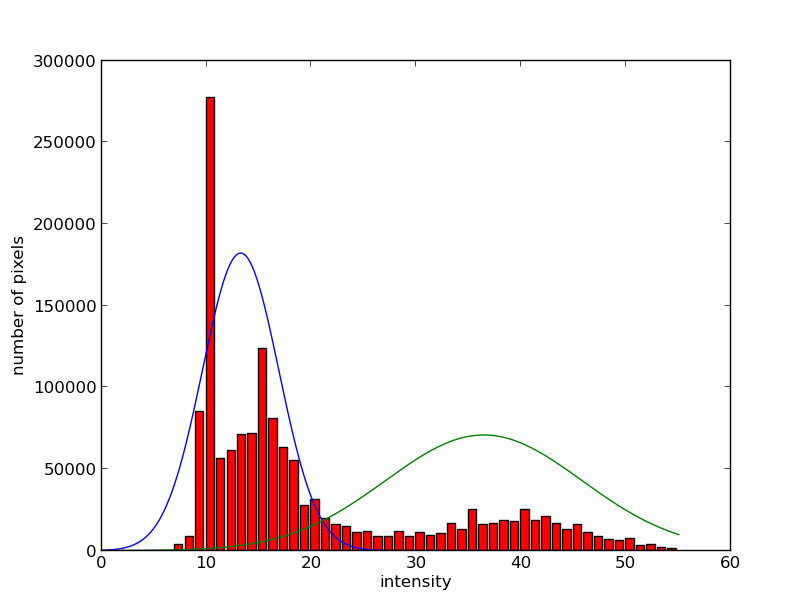
\includegraphics[scale=0.4]{Figures/segmentation/temp_hist_prez}
		\label{img:Approx}
		\caption{Approximation of an image histogram}
	\end{center}
\end{figure}

\begin{figure}
	\begin{center}
		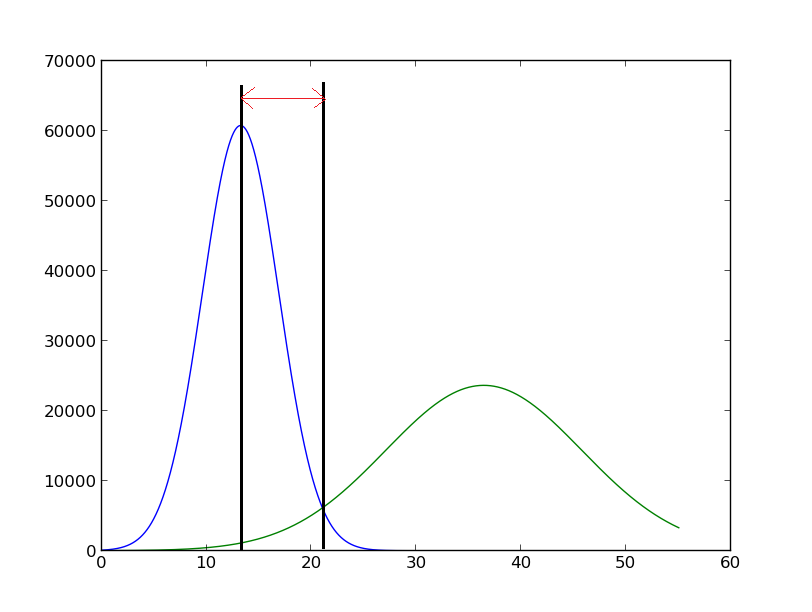
\includegraphics[scale=0.4]{Figures/segmentation/approx_hist_thr}
		\label{img:Thr}
		\caption{A calculation of a threshold}
	\end{center}
\end{figure}

The point of using the background segmentation step is to overcome a problem of undetected cells that expose a low intensity. To evaluate this step, the optimal threshold for each image in dataset was determined manually. The evaluation was perform in two ways - on object and pixel level. First, the number of detected cells was used as the number of cells in each image is known in advance. Second, segmented region were compared to the ground truth. As a measure of similarity \textit{precision} is used - number of pixels in segmented regions that is contained in the ground truth segmentation divided by the number of pixels in the ground truth segmentation. This measure should indicate a similarity of obtained segmentation to a manually segmented cells. \\

Table \ref{tab:Object} summarizes the object level results. The results show that the Region growing approach usually detects more objects than contained in the ground truth segmentation. Those extra object detected by the proposed approach are actually partial cells that were removed from the ground truth segmentation. The presences of those partial cells demonstrates the advantages and sensitivity of region growing, but also raises a question should those cells be eliminated from further process or used as a \textit{fully observed} cells.


%------------------------------------------------------%
%                                                      %
%               PRIOR POSITIONING                      %
%                                                      %
%------------------------------------------------------%

\section{Positioning a prior}

Once the background has been found, we have a rough estimate of cell positions. Still, a lot of cells overlap. In order to split them, we will make use of circularity properties of the cells. If circles of cells could be detected, or at least circular parts of cells, they might be split. To detect circles Hough transformation is used.

\subsection{Hough transformation for circles}

Hough transform is a general voting procedure used in Computer vision. The outline of the method is given in algorithm \ref{alg:Hough}. It discretize a parameter space and assigns every bin a number of votes proportional to the number of edges in an image that could be generated with that specific bin parameters. In our case, each bin represents one candidate circle in an image with equation 

\begin{equation}
	\mathcal{H}(\hat{x}, \hat{y}, r) = (\hat{x} - x)^2 + (\hat{y} - y)^2 = r^2,
\end{equation}

where  $\hat{x}$ and $\hat{y}$ represent the origin of a circle and $r$ its radius. Now every edge point in an image \textit{votes} for every bin that could have generated it, under assumption that the edge is a part of a circle. \\

\begin{algorithm}
	\caption{Hough Transform}
 	\label{alg:Hough}
 	\begin{algorithmic}[1]
 	\Function{Hough Transformation}{}
 		\State initialize accumulator $\mathcal{H}$ to all zeros
 		\For{ each edge in image }
 			\State increment every cell $\mathcal{H}(x,y,r)$ which could be the center of a circle
 		\EndFor
 		\State search for local maxima cells of $\mathcal{H}$
 	\EndFunction
\end{algorithmic}
\end{algorithm}

After voting, every local maximum is selected as a circle. Additionally, every vote could be weighted proportionally to its magnitude. Note that not all local maxima are actual circles. Although quite straightforward, the method can easily become unfeasible. Searching for all radius's is obviously unfeasible for large images, so any restriction on circle size range is most certainly helpful. To help the search, radius is limited to a range of minimal to the largest radius found in the data set. \\

Another problem with Hough transformation is its sensitivity to noise. If we assume there is an uniform noise in an image, it is easy to conclude that might imply false circles over an image. Methods to overcome that problem usually include better discretization of parameters or smoothing in the accumulator by incrementing neighboring bins, but for fully automated application this is not suitable solution. Instead, information about background extracted in the previous step could be used. As we can obtain background quite successfully, every circle with a center in the background region can be removed. so as every other circle which has similar properties as the background circles. As a criteria here, a mean intensity in the green channel is used - every circle with a mean intensity lower than the highest mean intensity found in the background is removed. Figure \ref{fig:Hough} illustrates that selection. Now each circle serves as a seed point for precise segmentation of contours and splitting overlapping cells.

\begin{figure}
	\begin{minipage}[h]{0.49\linewidth}
		\begin{center}
			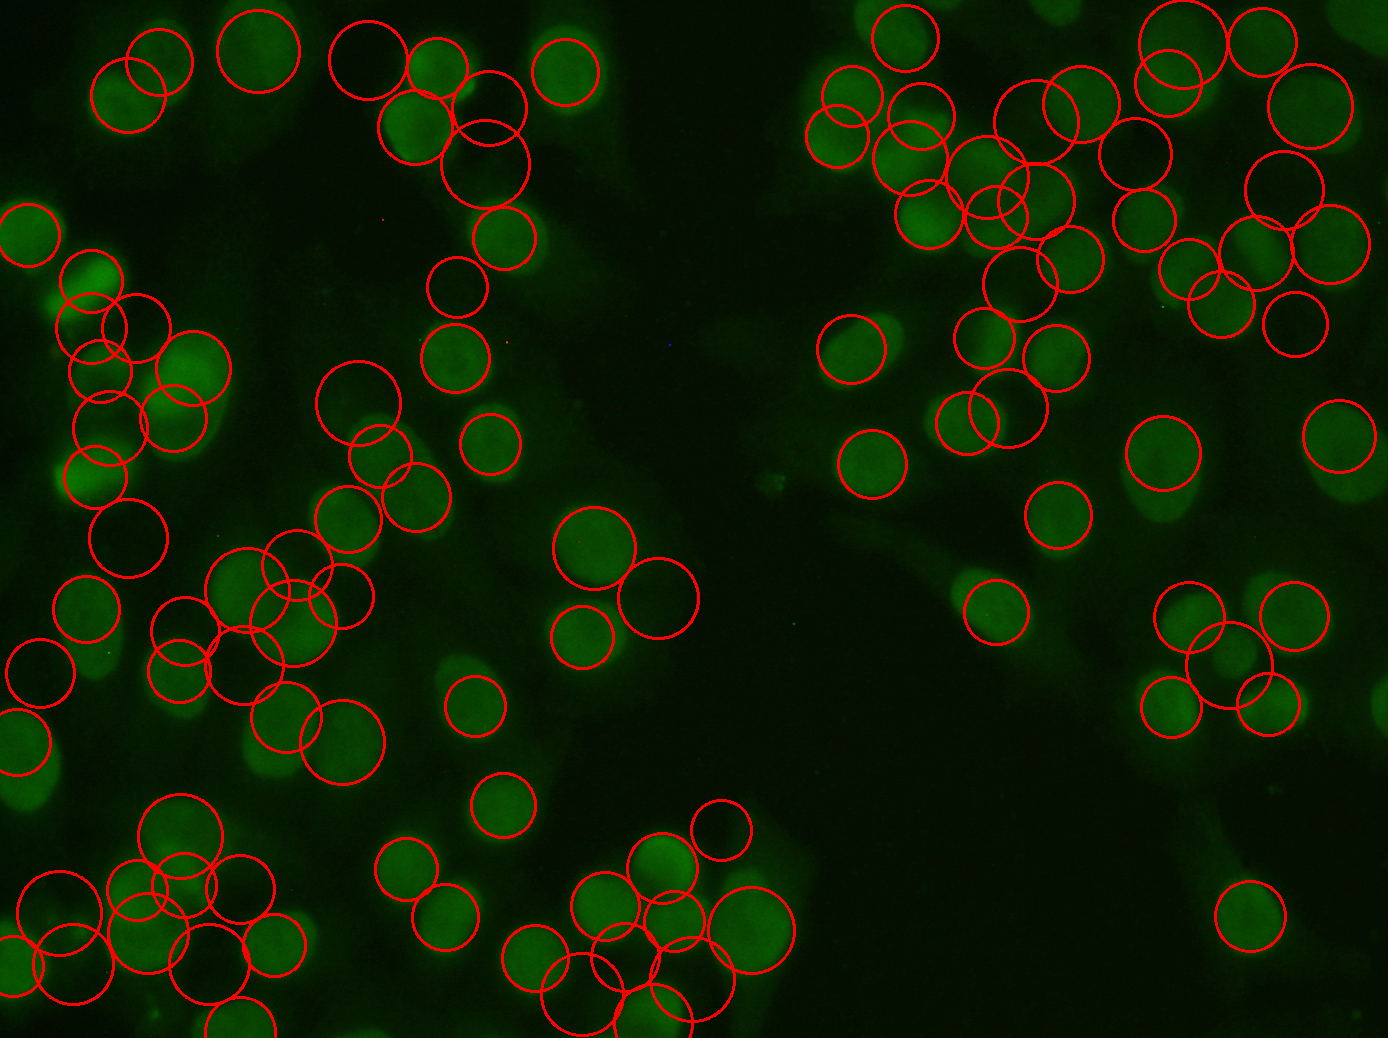
\includegraphics[scale=0.13]{Figures/segmentation/circles_no_selection}
			\\ (a)
		\end{center}	
	\end{minipage}
	\begin{minipage}[h]{0.49\linewidth}
		\begin{center}
			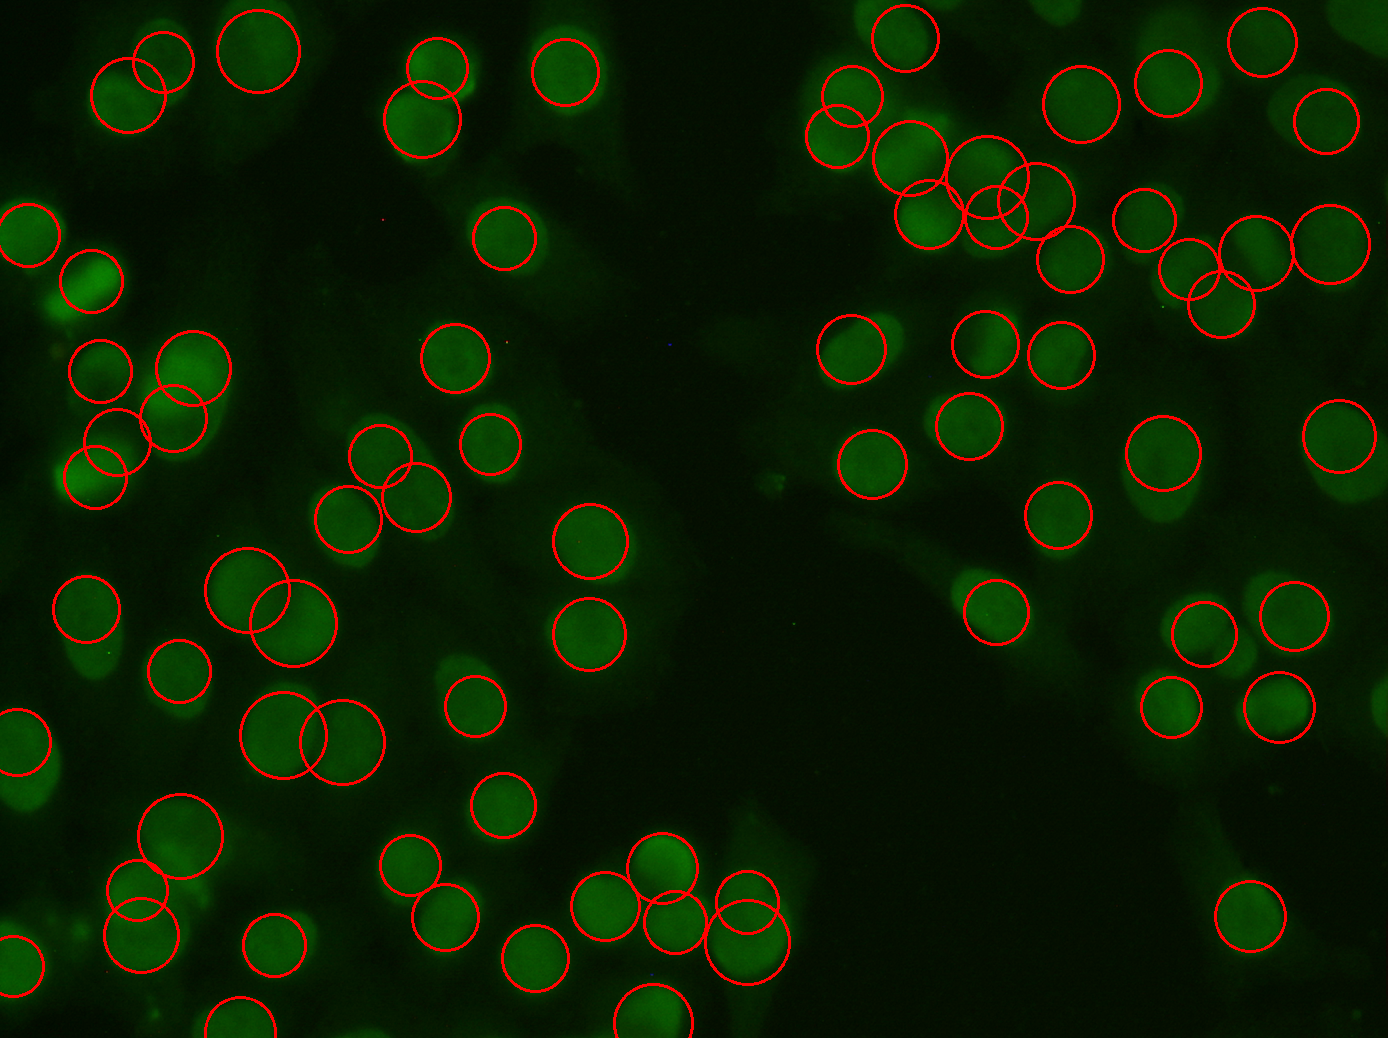
\includegraphics[scale=0.13]{Figures/segmentation/circles_after_selection}
			\\ (b)
		\end{center}
	\end{minipage}
	\caption{Hough transformation with all detected circles (a) and after removing background circles (b)}
	\label{fig:Hough}
\end{figure}

%-----------------------------------------------------%
%                                                     %
%             SEGMENTATION                            %
%                                                     %
%-----------------------------------------------------%

\section{Precise contours with Morphological snakes}

Morphological snakes or active contour methods are one very popular computer vision method. This method employs a energy optimization approach where it tries to minimize an energy functional induced by a curve.  The minimum is usually find by a steepest descent approach. \\

Here we are interested in a specific version of morphological snakes called \textit{Active contour without edges} (ACWE). The ACWE doesn't need well defined boarders and it is less sensitive to the initial configuration and model parameters. Due to a noisy nature of images used in this process, the ACWE has a potential to successfully deal with the noise. The Active contour methods try to adjust the starting contour to the local minimum by iteratively solving a time-dependent partial differential equations (PDE). However, solving the PDE is computationally costly and often has a stability issues. \\

The most efficient approaches avoid to solve the PDE directly. The key idea that allows the simplification of the problem is that the curve is implicitly  represented by the set of image points neighboring the target area. The evolution of curve is then achieved by elimination and introduction of points in the target set. Any geometric property can be approximated with local operations on the set of points. Those methods are based on mathematical morphology and make use of morphological operators such as \textit{erosion} and \textit{dilation} to approximate the PDEs. For the equivalence of differentiation and morphological operators see \cite{Pami2013}.




\subsection{Background }

This section summarizes the most important parts of curve evolution with PDEs and morphological operators.




\subsubsection{Contour evolution with PDEs}

Differential operators are key to contour evolution with PDEs -- the change of contour is given by a differential operator. \\

Let $\mathcal{C}$ be a parametrized 2D curve over time so that $\mathcal{C}: \mathbb{R}^+ \times [0,1] \rightarrow \mathbb{R}^2 : (t,p) \rightarrow \mathcal{C}(t,p)$. A differential operator $\mathcal{L}$ defines the curve evolution with PDE $\mathcal{C}_t = \mathcal{L}(\mathcal{C})$. The result of evolution depends on the differential operator. There are many forms in which it can be written but one popular is $\mathcal{L} = \mathcal{F} \cdot \mathcal{N}$, where $\mathcal{N}$ is the normal to the curve and $\mathcal{F}$ is a scalar field which determines the speed of evolution. \\

A particularly interesting form is the one in which $\mathcal{L}$ is defined with $\mathcal{F} \in \{ -1,1 \}$. Such operator evolves the curve along its normal direction with constant speed. If $\mathcal{F}$ takes the form of the Euclidean curvature of $\mathcal{C}$, then the problem is convex so it will converge to the optimal solution. \\

With the explicit representation of curve certain problems occur. It is not easy to deal with topological changes and re-parameterization of the curve. An alternative to the explicit representation is an implicit one. Let $u: \mathbb{R}^+ \times \mathbb{R}^2 \rightarrow \mathbb{R}$ an implicit representation of $\mathcal{C}$ such that $\mathcal{C}(t) = \{ (x,y); u(t,(x,y)) = 0 \}$. When $\mathcal{C}_t = \mathcal{F} \cdot \mathcal{N}$, the curvature evolution of any function $u(x,y)$ which embeds the curve is $\frac{\partial u}{\partial t} = \mathcal{F}|\nabla u|$. \\

With that in mind, the PDEs that are of interest to the curvature evolution are

\begin{equation}
	\frac{\partial u}{\partial t} = \pm |\nabla u|
	\label{eq:PDE1}
\end{equation}

\begin{equation}
	\frac{\partial u}{\partial t} = div \left ( \frac{\nabla u}{|\nabla u|}  \right ) \cdot |\nabla u|
	\label{eq:PDE2}
\end{equation}

where $\mathcal{F} = \pm 1$ in \ref{eq:PDE1} and $\mathcal{F} = \mathcal{K}$ for \ref{eq:PDE2}. $\mathcal{K}$ denotes the Euclidean curvature.



\subsubsection{Morphological operators} 

Morphological operators are monotone operators that are translation and contrast invariant. Every morphological operator $T$ can be represented in a $sup-inf$ representation of form 

\begin{equation}
	(T_hu)(\mathbf{x}) = \sup_{B \in \mathcal{B}} \inf_{\mathbf{y} \in \mathbf{x} + hB}u(\mathbf{y})
\end{equation}

or a dual $inf-sup$ form

\begin{equation}
	(T_hu)(\mathbf{x}) = \inf_{B \in \mathcal{B}} \sup_{\mathbf{y} \in \mathbf{x} + hB}u(\mathbf{y}),
\end{equation}

where $\mathcal{B}$ is a set of structuring elements that uniquely defines the operator and $h$ is the size of operator. \\

The most common morphological operators are dilation and erosion. A dilation $D_h$ with radius $h$ of function $u$ is defined as 

\begin{equation}
	D_hu(\mathbf{x}) = \sup_{\mathbf{x} \in hB(0,1)} u(\mathbf{x} + \mathbf{y})
\end{equation}

while the erosion has a similar form

\begin{equation}
	E_hu(\mathbf{x}) = \inf_{\mathbf{x} \in hB(0,1)} u(\mathbf{x} + \mathbf{y}),
\end{equation}

 where $B(0,1)$ is a ball of radius 1 centered at 0 and $h$ is the scaling factor.
 
\subsubsection{Curvature operator}

A curvature operator works as follows. Let $SI_h$ and $IS_h$ be respectively $sup-inf$ and $inf-sup$ morphological operators with a base $\mathcal{B}^2 = \{ [-1,1]_{\theta} \subset \mathbb{R}^2 : \theta \in [0, \pi) \}$. The base is made of all segments of length 2 centered at the origin. It can be proved that the successive application of \textit{a mean operator}, for a very small $h$, is equivalent to the curvature flow of PDE \ref{eq:PDE2}. \\

The mean operator is now defined as a composition of two morphological operators

\begin{equation}
	T_{h/2}^2 \ocircle T_{h/2}^1 \approx \frac{T_h^2u + T_h^1u}{2}.
\end{equation}

\subsection{Morphological snakes}
% Chapter Template

\chapter{Fluorescence intensity classification} % Main chapter title

\label{Chapter5} % Change X to a consecutive number; for referencing this chapter elsewhere, use \ref{ChapterX}


%----------------------------------------------------------------------------------------
%	INTRODUCTION
%----------------------------------------------------------------------------------------

The fluorescence intensity is a parameter that describes the \textit{clarity} of cells in image. It is a subjective parameter which, unfortunately, doesn't have a strong theoretical explanation. The fluorescence intensity is described with three values - positive, intermediate and negative. Positive value defines images in which cells are perfectly separated from background, while negative value defines images in which cells in which cells cannot be identified. The intermediate value covers images that are not positive nor negative. This parameter is used as a symbolic feature later in the process, but for the sake of \textit{standard procedure} it is estimated separately. \\


In \cite{Rigon2007} Rigon studied the variability of decision made by doctors and showed that it is hard to achieve a consensus about unique determination of the fluorescence intensity value. The lack of underlying model is making this problem hard to formulate. The intuition behind the suggested approach is an assumption that intensity level could be observed in the histogram of an image. The fluorescence intensity should correspond to the difference to a region describing the background and a region describing cells. Following the intuition, an image histogram is approximated with the Gaussian mixture model. \\

The idea is to approximate the histogram with a mixture of two Gaussian functions - one representing the background and second one to model the cells. The intuition is that images with positive intensity should have Gaussians with higher means and more further apart. 


%-----------------------------------------------------------------------------------------
%     Classifying intensity
%-----------------------------------------------------------------------------------------

\section{Classifying intensity}

Once histogram has been approximated with two Gaussian functions, the estimated means and variances have taken as features for the classification. SVM with radial basis functions as kernel function has been trained for the task. Evaluation is performed using a 10-fold cross validation. \\



%--------------------------------------------------%
%                                                  %
%               SVM                                %
%                                                  %
%--------------------------------------------------%


\subsection{Support Vector Machine}


Support vector machine is a very popular machine learning technique. It is a representative of a more general class of \textit{kernel methods}. The most interesting property of the support vector machine is that it tries to find the \textit{optimal hyperplane} that separates classes. Consider a two-class case. The sample is $\mathcal{D} = \{ \mathbf{x}^{(i)}, y^{(i)} \}_{i=1}^N$ where $y^{(i)} = 1$ if $\mathbf{x}^{(i)} \in \mathcal{C}_1$ and $y^{(i)} = -1$ if $\mathbf{x}^{(i)} \in \mathcal{C}_2$. We want to find a margin $\mathbf{w}$ so that

\begin{equation*}
	\mathbf{w}^T\mathbf{x}^{(i)} + w_o \geq +1 \quad \mathtt{for} \quad y^{(i)} = 1
\end{equation*}

\begin{equation*}
	\mathbf{w}^T\mathbf{x}^{(i)} + w_o \leq -1 \quad \mathtt{for} \quad y^{(i)} = -1
\end{equation*}

or simplified 

\begin{equation*}
	y^{(i)}(\mathbf{w}^T\mathbf{x}^{(i)} + w_0) \geq 1.
\end{equation*}

The support vector machine extends the \textit{basic} hyperplane requirement - setting the instances on the right side of the hyperplane - by trying to maximize the margin - the distance from the hyperplane to the instances closest to it. So, the \textit{optimal separating hyperplane} is the one that maximizes the margin. \\

The distance of $\mathbf{x}^{(i)}$ to the hyperplane equals to 

\begin{equation}
	\frac{ | \mathbf{w}^T\mathbf{x}^{(i)} - w_0 | }{ \Vert \mathbf{w} \Vert}.
\end{equation}

Finding the maximal margin can be expressed as

\begin{equation}
	\frac{y^{(i)}(\mathbf{w}^T\mathbf{x} - w_0)}{\Vert \mathbf{w} \Vert} \geq \rho, \forall i,
\end{equation}

i.e., we want the margin to be at least $\rho$. As there are infinitely many solutions that can be obtained by scaling $\mathbf{w}$, we fix the $\rho \Vert \mathbf{w} \Vert = 1$ and minimize $\Vert \mathbf{w} \Vert$ to maximize the margin. The problem can now be written in a form of quadratic optimization problem

\begin{align*}
	\min_{\mathbf{w}, w_0} & \quad \frac{1}{2} \Vert \mathbf{w} \Vert \\
	\mathtt{subject \ to} & \quad  y^{(i)} \left ( \mathbf{w}^T\mathbf{x} + w_0  \right ) \geq 1.
\end{align*}

Now there will be instances that are $\frac{1}{\Vert \mathbf{w} \Vert}$ away from the hyperplane and the total margin equals to $\frac{2}{\Vert \mathbf{w} \Vert}$. \\

If the problem is not linearly separable, one trick is to map the problem to a new space, with more dimension that the original space, by using nonlinear basis functions. It is generally the case that higher dimensional representation is easier to separate. One such mapping function is the \textit{radial basis function}. 


%---------------------------------------%
%                                       %
%                RBF                    %
%                                       %
%---------------------------------------%
 
\subsection{Radial basis functions}

Radial basis functions are an instance of a \textit{local representation}, where for a given input, only a few factors are \textit{active}. It is in a way a partition of a space so that \textit{locally tuned} partitions are selective to only certain inputs. \\

With the concept of local partitioning we need to define a measure of similarity between an input $\mathbf{x}^{(i)}$ and the local clusters $\boldsymbol \mu^1, \ldots, \boldsymbol \mu^n$. The radial basis functions are defined as

\begin{equation}
	\mathbf{r}(\mathbf{x}^{(i)}, \boldsymbol \mu^k) = exp \left (- \frac{\Vert \mathbf{x}^{(i)}  - \boldsymbol \mu^k \Vert}{2\sigma_k^2} \right ),
\end{equation} 

that is, it uses the Euclidean distance as a measure of similarity and Gaussian function as a response function. The response function express a property of having a maximum where $\mathbf{x}^{(i)} = \boldsymbol \mu^k$ and decreasing as they get less similar. 




%--------------------------------------%
%                                      %
%           EVALUATION                 %
%                                      %
%--------------------------------------%

\subsection{Results}

One issue that might occur is a bad estimation of the background or cell body as some cells takes a very small portion of an image or, on the other size, takes almost a whole image when segmented as shown in image \ref{fig:Bad}. To see how this influences the problem, histograms are approximated with Gaussian functions in two ways. First, the histogram is as in Chapter \ref{Chapter4}, without any restrictions. Second, the background and cells part of an image are separated and each part is approximated with a Gaussian individually. \\

\begin{figure}
	\begin{minipage}[h]{0.32\linewidth}
		\begin{flushright}
			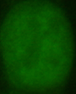
\includegraphics[height=2cm]{Figures/intensity/image1}
		\end{flushright}
	\end{minipage}
	\begin{minipage}[h]{0.32\linewidth}
		\centering
		
\includegraphics[height=2cm]{Figures/intensity/image2}
	\end{minipage}
	\begin{minipage}[h]{0.32\linewidth}
		\begin{flushleft}
			
\includegraphics[height=2cm]{Figures/intensity/image3}
		\end{flushleft}
	\end{minipage}
	\caption{Potential image that could obtain bad estimation}
	\label{fig:Bad}
\end{figure}

Table \ref{res:SepReg} summarizes the results obtained with separation of background and cell regions (a) and without (b). The accuracy of proposed solution is 96.21 \% and 96.08 \% for separation and without it, respectively. As the results for both cases don't show any significant difference, the stability of method is promising.  The best performance reported so far is 92,6 \% although the authors have used a private data set that is not available online, so it is hard to make a comparison.  So far, the results of this data set are not yet reported. \\

The evaluation is performed on cell level - the intensity level is estimated on cell level. In practice, the intensity level is assigned on image level. Each cell in the image is then assigned with a level of the image. Averaging the classification over an image, a 100 \% accuracy is achieved.




\begin{figure}
	\caption{Results of intensity classification}
	\label{res:SepReg}
	\begin{minipage}[h]{0.49\linewidth}
		\begin{center}
			\begin{tabular}{c c| c c}
				 & & \multicolumn{2}{c}{True} \\
			     & & \textbf{pos} & \textbf{int} \\
			    \hline
			    \multirow{2}{*}{\rotatebox[origin=c]{90}{Pred}} & \textbf{pos} & 804 & 31 \\
			    & \textbf{int} & 25 & 595
			\end{tabular} \\
		a)
		\end{center}
	\end{minipage}
	\begin{minipage}[h]{0.49\linewidth}
		\begin{center}
			\begin{tabular}{c c| c c}
				 & & \multicolumn{2}{c}{True} \\
			     & & \textbf{pos} & \textbf{int} \\
			    \hline
			    \multirow{2}{*}{\rotatebox[origin=c]{90}{Pred}} & \textbf{pos} & 800 & 36 \\
			    & \textbf{int} & 29 & 590
			\end{tabular} \\
			b)
		\end{center}
	\end{minipage}
\end{figure}


% Chapter Template

\chapter{Describing cells} % Main chapter title

\label{Chapter6} % Change X to a consecutive number; for referencing this chapter elsewhere, use \ref{ChapterX}


Once cells have been segmented and their fluorescence intensities classified, there are assigned with features that describe a human perception of the cells' properties. The interesting properties are summarized in the following section. 


%----------------------------------------------------------------------------------------
%	FEATURES
%----------------------------------------------------------------------------------------

\section{Interesting features}




%--------------------------------------------%
%                                            %
%             DEEP LEARNING                  %
%                                            %
%--------------------------------------------% 

\section{Deep learning}





%--------------------------------------------%
%                                            %
%           DEEP BELIEF NETWORKS             %
%                                            %
%--------------------------------------------%

\section{Deep belief networks}





%--------------------------------------------%
%                                            %
%               EVALUATION                   %
%                                            %
%--------------------------------------------%

\section{Evaluation}


% Chapter Template

\chapter{Rule mining} % Main chapter title

\label{Chapter7} % Change X to a consecutive number; for referencing this chapter elsewhere, use \ref{ChapterX}


\texttt{IF-THEN} rules are the most natural way of expressing knowledge. They are easy to understand and quite expressive. Because of their nature to represent knowledge, mining knowledge in such form is of interest to this project. \\

The symbolic representation of cells obtained in the previous step is here used as an input features. Two popular approaches for mining such rules in a supervised way are \textit{Decision trees} and \textit{Inductive Logic Programming}.



%----------------------------------------
% DECISION TREE
%----------------------------------------

\section{Decision Trees}

Decision trees are one popular instance of machine learning algorithms due to their \textit{simplicity} and \textit{interpretability}. The decision tree approximates discrete functions and it is very robust to noisy data which makes it suitable for this application. It uses the \textit{tree} structure to represent and compress the data where each \textit{node} represents a test on attribute and each \textit{branch} stands for values of the tested attribute. \\

The decision tree performs a \textit{greedy search} in a search space and chooses an attribute to split data on. The chosen attribute then becomes the node in the tree, and values it can take become branches. As a measure of \textit{quality} of an attribute, \textit{information gain} is used. \\

Information gain compares the \textit{entropy} of the dataset before and after splitting. For a $K$ class case, entropy of data set $\mathcal{D}$ is defined as

\begin{equation}
	\mathtt{Entropy}(\mathcal{D}) = \sum_{k=1}^K p(\mathcal{C}_k)\mathtt{log}_2 p(\mathcal{C}_k)
\end{equation}

where $p(\mathcal{C_k})$ stands for a fraction of examples in data set $\mathcal{D}$ that belong to class $\mathcal{C}_k$. Informally, it measures the \textit{impurity} of data. Having entropy defined, information gain achieved by splitting on attribute $A$ is defined as

\begin{equation}
	\mathtt{InformationGain}(\mathcal{D}, A) = \mathtt{Entropy}(\mathcal{D}) - \sum_{v \in values(A)} \frac{\vert \mathcal{D}_v \vert}{\vert \mathcal{D} \vert}\mathtt{Entropy}(\mathcal{D}_v)
\end{equation} 

where $\mathcal{D}_v = \{ x \in \mathcal{D} | A(x) = v \}$ represents a subset of the original data set $\mathcal{D}$ with attribute $A$ equal to $v$. Informally, as entropy measures the \textit{impurity} of data, information gain measures how much of the \textit{impurity} has been lost by splitting the data. The partitioning continues until there are not attributes to split on, or the data contains only examples for the same class. Decision trees are summarized in Algorithm \ref{alg:DT}.


\begin{algorithm}
	\caption{Decision Tree learning}
	\label{alg:DT}
	\begin{algorithmic}[1]
		\Function{DecisionTree}{$\mathcal{D}$, \textbf{X}}
			\State $T \gets$ new tree
			\If{ all instances in $\mathcal{D}$ have same class $c$}
				\State $\mathtt{Label}(T) = c$
				\State return $T$
			\EndIf	
			\If{ \textbf{X} = \o}
				\State $\mathtt{Label}(T) = $ most common class in $\mathcal{D}$
				\State return $T$
			\EndIf 
			\State $X \gets$ attribute with highest information gain
			\State $\mathtt{Label}(T) = X$
			\For{ each $x$ in \textbf{X}}
				\State $\mathcal{D}_x \gets $ examples from $\mathcal{D}$ with $X = x$
				\If{$\mathcal{D}_x$ is empty}
					\State let $T_x$ be a new tree
					\State $\mathtt{Label}(T_x) \gets $ most common class in $\mathcal{D}_x$
				\Else
					\State $T_x \gets \text{ DecisionTree}(\mathcal{D}_x, \mathbf{X} - \{ X \})$
				\EndIf
				\State add a branch from $T$ to $T_x$
			\EndFor
			\State return $T$
		\EndFunction 
	\end{algorithmic}
\end{algorithm}

%----------------------------------------------------------------------------------------
%	ILP
%----------------------------------------------------------------------------------------

\section{Inductive logic programming}

Inductive logic programming (ILP) is an intersection between Machine learning and Logic programming where logic representation is used to induce knowledge. Inductive logic programming is concerned with finding a hypothesis $\mathcal{H}$ from a set of positive and negative examples $\mathcal{P}$ and $\mathcal{N}$. It is required that the hypothesis $\mathcal{H}$ covers all positive examples in $\mathcal{P}$ and none of the negative examples in $\mathcal{N}$. \\

ILP programs incorporate \textit{background knowledge} to induce rules from positive examples. It is convenient to view the background knowledge $\mathcal{B}$ as a logic program that is provided to the ILP system and fixed during the learning process. Under the presence of background knowledge, the hypothesis $\mathcal{H}$, together with the background theory $\mathcal{B}$, should cover all positive and none of the negative examples. \\

Many ILP systems have been developed over the years and three representative systems are described here.

\subsection{FOIL}

FOIL algorithm is an instance of \textit{Sequential covering} algorithms. Sequential covering employs the \textit{divide-and-conquer} principle and tries to learn one rule at time. Every induce rule should cover as many positive examples as possible, and as less negative examples as possible. \\

FOIL is summarized in Algorithm \ref{alg:FOIL}. FOIL performs a general-to-specific search where each candidate clause to a current rule is in one of the following forms:

\begin{itemize}
	\item $\mathcal{Q}(v_1,\ldots, v_n)$ where $\mathcal{Q}$ is a predicate from the set of all predicates and $v_i$ are either variables already present in the rule or new variables
	\item $\mathtt{Equal}(x_i, x_j)$ where $x_i \text{ and } x_j$ are variables already present in the rule
	\item the negation of either of the above mentioned forms.
\end{itemize}

Another important step in FOIL is the evaluation of candidate clauses. Let $R'$ be the rule created by adding candidate clause $L$ to rule $R$. Performance measure $\mathtt{FoilGain}(L,R)$ is defined as

\begin{equation}
	\mathtt{FoilGain}(L,R) = t \left ( \mathtt{log}_2 \frac{p_1}{p_1 + n_1} - \mathtt{log}_2 \frac{p_0}{p_0 + n_0} \right ),
\end{equation}

where $p_0$ stands for the number of positive bindings of rule $R$, $n_0$ is the number of negative bindings of $R$, while $p_1$ and $n_1$ represent the number of positive and negative bindings of $R'$. 

\begin{algorithm}
	\caption{FirstOrderInductiveLearner}
	\label{alg:FOIL}
	\begin{algorithmic}[1]
		\Function{FOIL}{examples}
			\State \textit{Pos} $\gets$ a set of \textbf{positive} examples
			\State \textit{Neg} $\gets$ a set of \textbf{negative} examples
			\State \textit{LearnedRules} $\gets \{ \}$ 
			\While{\textit{Pos}}
				\State \textit{NewRule} $\gets$ LearnRule()
				\State \textit{LearnedRules} $\gets$ \textit{LearnedRules} $+$ \textit{NewRule}
				\State \textit{Pos} $\gets$ \textit{Pos} - \{ covered positive examples \}
			\EndWhile
			\State return \textit{LearnedRules}
		\EndFunction
		\Statex
		\Function{LearnRule}{}
			\State \textit{NewRule} $\gets$ the empty rule that predict the \textit{target} attribute
			\State \textit{NewRuleNeg} $\gets$ \textit{Neg}
			\While{NewRuleNeg}
				\State \textit{CandidateLiterals} $\gets$ generate candidate literals for \textit{NewRule}
				\State \textit{BestLiteral} $\gets  \arg\max_{L \in CandidateLiterals}FoilGain(L, NewRule)$
				\State add \textit{BestLiteral} to precondition of \textit{NewRule}
				\State \textit{NewRuleNeg} $\gets$ subset of \textit{NewRuleNeg} covered by \textit{NewRule}
			\EndWhile		
		\EndFunction
	\end{algorithmic}
\end{algorithm}







\subsection{RIPPER}

The RIPPER algorithm is another instance of the sequential covering algorithms. Compared to FOIL, it introduces two additional steps - rule pruning and rule optimization. The algorithm is summarized in Algorithm \ref{alg:RIPPER}. \\

For multi-class problems, it orders the classes according to increasing class prevalence --  a fraction of instances that belong to a particular class. It learns the rule set for the smallest class first and treats other classes as negative. It then repeats the process taking the next smallest class as a positive class. RIPPER also uses $\mathtt{FoilGain}$ measure as the performance measure.\\

The pruning step is done by using \textit{Incremental Reduced Error Pruning}. The data set is split into the training and validation set. The rule is then induced from the training set. The validation set is used to prune the rules. For each rule, performance measure $v$ is calculated with a precondition removed. The performance measure $v$ is defined as 

\begin{equation}
	v(pruneRule, Pos, Neg) = \frac{p - n}{p + n},
\end{equation}

where $p$ is the number of positive examples in the validation set covered by the pruned rule and $n$ is the number of negative examples in the validation set covered by the pruned rule. \\

In the optimization step, for each rule two new rules are generated. One is completely built from scratch while the second one is generated by adding new conjunctions to the existing rule. As RIPPER performs the greed search, the rule built from scratch might not be the same as the starting one. In that way, three separate rule sets are generated and compared. The resulting rule set is chosen to minimize the \textit{Minimum Description Length} (MDL). MDL uses the assumption that any \textit{regularity} in the data can be used to \textit{compress} the data. Given the hypothesis' set $\mathcal{H}^{(0)}, \mathcal{H}^{(1)}, \ldots, \mathcal{H}^{(n)}$, which in this case are the rule sets, the best hypothesis is the one which minimizes the distance 

\begin{equation}
	L(\mathcal{H}) + L(\mathcal{D} | \mathcal{H}),
\end{equation}

where $L(\mathcal{H})$ is the length, in bits, of the description of the hypothesis and $L(\mathcal{D} | \mathcal{H})$ is the length, in bits, of the description of data when encoded with the help of the hypothesis.


\begin{algorithm}
	\caption{RIPPER}
	\label{alg:RIPPER}
	\begin{algorithmic}[1]
		\Function{RIPPER}{examples, predicates}
			\State \textit{LearnedRules} $\gets \{ \}$
			\State order classes in ascending order according to their prevalence
			\State \textit{CurrentClass} $\gets$ smallest class
			\State \textit{Pos}, \textit{Neg} $\gets$ positive and negative examples of \textit{CurrentClass}
			\While{\textit{Pos}}
				\State split data set into \textit{training} and \textit{validation} set
				\State \textit{NewRule} $\gets$ LearnRule(\textit{training set})
				\State \textit{NewRule} $\gets$ PruneRule(\textit{validation set}, \textit{NewRule})
				\State \textit{LearnedRules} $\gets$ \textit{LearnedRules} + \textit{NewRule}
				\State remove examples covered by \textit{NewRule}
				\State \textit{CurrentClass} $\gets$ smallest class after removing examples
				\State \textit{Pos}, \textit{Neg} $\gets$ positive and negative examples of \textit{CurrentClass}
			\EndWhile
			\State Optimize(\textit{LearnedRules})
			\State return \textit{LearnedRules}
		\EndFunction
		\Statex
		
		\Function{LearnRule}{\textit{Pos}, \textit{Neg}}
			\State \textit{Rule} $\gets \{ \}$
			\While{ there are \textit{Neg} covered}
				\State add conjunct if it improves $\mathtt{FoilGain}$
			\EndWhile
			\State return \textit{Rule}
		\EndFunction
		\Statex
		
		\Function{Prune}{\textit{Pos}, \textit{New},\textit{Rule}}
			\Repeat
				\State \textit{Predicate} $\gets$ select a precondition from \textit{Rule}
				\State $v(pruneRule,Pos,Neg) = \frac{p - n}{p + n}$
				\State delete \textit{Predicate} if it improves $v$ 
			\Until{no deletion improves $v$}
		\EndFunction
		\Statex
		
		\Function{Optimize}{Rules}
			\For{each rule $r$ in \textit{Rules}}
				\State replacement rule $r* \gets$ build new rule
				\State revised rule $r' \gets$ add conjuncts to extend $r$
				\State compare the rule set for $r$ against the rules set for $r*$ and $r'$
				\State choose the rule set that minimizes the MDL
			\EndFor
		\EndFunction
	\end{algorithmic}	

\end{algorithm}






\subsection{Aleph}

\texttt{Aleph} (\textbf{A} \textbf{L}earning \textbf{E}ngine for \textbf{P}roposing \textbf{H}ypotheses) is another commonly used rule induction system. The outline of the approach is summarized in Algorithm \ref{alg:Aleph}.  \\

It starts with a selection of an example to generalize. When the examples is selected, the most specific clause is built. The constructed clause has to entail the selected example and it is usually a \textit{bottom clause} -- a definite clause with many literals. \\

\texttt{Aleph} then performs a search to generalize the bottom clause. Generalization is done by searching for a subset of the literals in the bottom clause that score the best. The search is performed by a \textit{branch-and-bound} search. At this moment \texttt{Aleph} tries to find the best generalization of the current bottom clause, although it does not produce all generalizations. When the best clause is found, it is added to the current theory and all examples covered by the clause are removed. \\

The generalization of a clause is summarized in the function \texttt{GENERALIZE} in Algorithm \ref{alg:Aleph}. It starts by selecting a clause from the \textit{active set}. Clauses are selected in a way that clauses with fewer literals are chosen first. The selected clause is then \textit{branched} by adding one literal at time. For each child, the cost and lower bound are calculated. Lower bounds represent the lower cost that can be obtained at the node (that represent the clause) and the sub-tree below it. 

\begin{algorithm}
	\caption{Aleph}
	\label{alg:Aleph}
	\begin{algorithmic}[1]
		\Function{Aleph}{examples}
			\State \textit{Pos} $\gets$ positive examples
			\State \textit{Neg} $\gets$ negative examples
			\State \textit{theory} $\gets \{ \}$
			\While{\textit{Pos}}
				\State \textit{example} $\gets$ select example
				\State \textit{clause} $\gets \mathtt{BuildMostSpecificClause}$(\textit{example}) 
				\State \textit{rule} $\gets \mathtt{Generalize}$(\textit{clause})
				\State \textit{theory} $\gets$ \textit{theory} $+$ \textit{rule}
				\State Remove redundant
			\EndWhile
		\EndFunction
		\Statex
		\Function{Generalize}{examples,clause}
			\State \textit{activeSet} $\gets$ \{ 0\}
			\State \textit{Cost} $\gets \infty $
			\State \textit{CurrentBest} $\gets$ select random
			\While{\textit{activeSet} contains clauses}
				\State remove first node $k$ from \textit{activeSet}
				\State generate children of $k$, compute costs $Cost_i$ and lower bounds on costs $L_i$
				\For{each child}
					\If{$L_i > C$}
						\State prune child
					\Else						
						\If{child is complete solution \texttt{AND} $Cost_i < C$}
							\State $Cost \gets Cost_i$
							\State \textit{CurrentBest} $\gets$ child
							\State prune clauses in \textit{activeSet} with $L_i$ more than $Cost_i$ 
						\EndIf
						\State add child to \textit{activeSet}
					\EndIf
				\EndFor
			\EndWhile 
		\EndFunction
	\end{algorithmic}
\end{algorithm}


\section{Results and induced rules}

The above described methods are used to extract rules that describe the patterns. Classifiers are evaluated with the 10-fold cross validation. Tables \ref{tab:Perf} summarizes the precision and recall of each classifier. Results are represented class-wise together with the number of rules found. \\

When analyzing the performance of the classifier, both accuracy and the number of induced rules should be considered. The results suggest that Decision trees and RIPPER perform the best. The overall accuracy of the decision tree and RIPPER are 95.26 \% and 94.50 \% respectively. The decision tree achieves the highest accuracy, but produces significantly  more rules - 25 compared to 10 induced by RIPPER. Such a difference suggests  overfitting. Induced rules are shown in Appendix \ref{AppendixB}. It can be observed that RIPPER not only produces less rules, but those rules are also much simpler than ones induced by the decision tree. Rules induced by RIPPER usually have one or two clauses in the body, while rules induced by the decision tree usually have three or four clauses in the body. Also, it can be seen that 9 out of 25 rules induced cover less than 10 examples in the dataset. The state-of-the-art performance reported so far is 95.19 \% \cite{Wiliem}. The obtained results are quite comparable to their work, but also provide explainable results.\\

An interesting result is that \texttt{Aleph} for most patterns has the highest precision, but significantly lower recall. Moreover, an interesting case is a recognition of the \textit{coarse speckled} class which has very bad performance where only one percent of patterns is classified correctly. The other algorithms obviously don't have any problem with classification of the coarse speckled pattern. \\

Taking both performance and simplicity into account, the rules induced by RIPPER seem to perform the best. Their simplicity makes them more applicable to real life scenarios. They also correspond more to the intuition about the patterns. The induced rules mostly extract the most distinguishing property of a certain pattern. For example, \textit{centromere} class is identified by a large number of objects in the cell body, \textit{cytoplasmatic} by the irregular shape and \textit{coarse speckled} by rough texture. All of these properties are characteristic for specific patterns and don't appear for other types. The drawback of this approach is that rules should be always applied \textit{sequentially}. \\

As suggested in the literature, the most difficult classes to classify are \textit{fine speckled} and \textit{homogeneous}. It is very hard to distinguish between those two classes because they look very similar, especially in low intensity images. The literature indicated that mitotic cells are highly informative for this task. It appears that  \texttt{RIPPER} and \texttt{decision trees} are able to capture those relations, while \texttt{ALEPH} and \texttt{FOIL} are not. \\

Table \ref{tab:FulSys} summarizes the results obtained when features generated by the deep belief network is used. The performance of \texttt{Decision tree} in this case equals 91.34 \%, while \texttt{RIPPER} classifies 90.51 \% of the cells correctly. An interesting observation is that, although the deep belief network misclassifies approximately 10 \% of symbolic features, the effect is reduced by the redundancy in the symbolic features. The features that have the lowest recognition rate mostly belong to the patterns with a specific mitotic cells. For example, the large number of organelles is characteristic for the \textit{centromere} pattern, which is the only pattern that has the sparkly mitotic cells. 


\begin{table}
	\scriptsize
	\caption{Performance of the classifiers}
	\label{tab:Perf}
	\begin{tabular}{|c|c|c||c|c||c|c||c|c|}
		\hline
		& \multicolumn{2}{c}{\texttt{Decision tree}} & \multicolumn{2}{c}{\texttt{RIPPER}} & \multicolumn{2}{c}{\texttt{FOIL}} & \multicolumn{2}{c}{\texttt{Aleph}} \\
		\textbf{pattern} & Prec & Rec & Prec & Rec & Prec & Rec & Prec & Rec \\
		\hline \hline
		homogeneous & 93.48 \% & 100 \% & 93.48 \% & 100 \% & 92.15 \% & 100 \% & 100 \% & 69.69 \% \\
		nucleolar & 97.10 \% & 97.10 \% & 94.65 \% & 95.44 \% & 97.10 \% & 88.78 \% & 97.75 \% & 72.19 \%\\
		centromere & 100 \% & 93.56 \% & 98.24 \% & 93.54 \% & 100 \% & 92.37 \% & 100 \% & 93.22 \%\\
		cytoplasmatic & 96.46 \% & 100 \% & 96.33 \% & 96.33 \% & 96.46 \% & 90.9 \% & 100 \% & 100 \% \\
		fine speckled & 87.00 \% & 93.27 \% & 83.33 \% & 86.54 \% & 87.00 \% & 58.57 \% & 99.09 \% & 52.4 \%\\
		coarse speckled & 88.10 \% & 96.86 \% & 92.78 \% & 85.71 \% & 96.86 \% & 84.27 \% & 40 \% & 1 \%\\
		\hline \hline
		\textbf{\#rules} & \multicolumn{2}{c}{25} & \multicolumn{2}{c}{10} & \multicolumn{2}{c}{17} & \multicolumn{2}{c}{18} \\
		\hline
	\end{tabular}
\end{table}

\begin{table}
	\caption{Performance with features from DBN}
	\label{tab:FulSys}
	\small
	\begin{tabular}{|c c||c|c|c|c|c|c|}
		\hline
		& & homogeneous & nucleolar & centromere & cytoplasmatic & fine speckled & coarse speckled \\
		\hline
		\multirow{2}{*}{\rotatebox[origin=c]{90}{\tiny RIPPER}} & Prec & 92.94 \% & 86.40 \% & 94.67 \% &  98.02 \% & 81.40 \% & 90.91 \% \\
		 & Rec & 99.70 \% & 92.95 \% & 89.64 \% & 90.83 \% & 84.13 \% & 80.95 \% \\
		 \hline
		  \multirow{2}{*}{\rotatebox[origin=c]{90}{DT}} & Prec & 92.94 \% & 90.94 \% & 99.70 \% & 98.98 \% & 79.05 \% & 84.47 \% \\
		   & Rec & 99.70 \% & 95.85 \% & 93.00 \% & 88.90 \% & 79.81 \% & 82.86 \% \\
		   \hline
	\end{tabular}
\end{table}






\chapter{Conclusion}

\label{Conclusion}

This thesis proposes a solution for computer aided assistance in commonly used diagnostics in autoimmune diseases. The solution closely follows the procedure medical experts suggest. It covers the segmentation task,  the fluorescence intensity level classification and staining pattern classification. The strongest contribution of this thesis is the interpretable approach to prediction models that help medical experts. \\

The work on the segmentation part was motivated by two problems found in previous approaches. Due to the coloring procedure of fluorescence imaging, cells exhibit different properties which makes them hard to detect, especially in noisy images. By finding the background instead of cells directly, that problem was successfully solved with great improvement. Still, a lot of cells overlap.  By using the information about the background, morphological snakes were introduced. Although not always capable of separating overlapping cells, the method demonstrated very promising results. The problematic case were the patterns with bright organelles where those organelles were segmented. \\

The cells were then characterized with \textit{visual concepts} describing their appearance. Deep belief networks were used to map images, or pixel features to \textit{symbolic} ones. Deep approaches to machine learning demonstrated the great potential in symbolic feature recognition. Surprisingly, convolutional components seem not to improve the recognition, but the full potential of this approach is yet to be investigated. \\

The symbolic representations learned in the previous step are then used to mine rules that describe the patterns. Four commonly used rule mining algorithms were compared and proven to perform as accurately as state-of-the-art methods, but offer explanations about their decisions. I believe such an approach is needed when computers assist in making a diagnosis, based on images or other diagnostic tests.

\begin{flushleft}
	\large
	\vspace{15pt}
	\textbf{Future work}
\end{flushleft}

In order to make a fully functional system that supports this process, there are still problems that need to be solved. The segmentation task still suffers from certain problems, such as \textit{overexposed} organelles in a cell's body which end oversegmented. Introducing a model based segmentation method, where movement of the contour is restrained by model learned from data, might be a way to improve the segmentation of cells. \\

There are two actions that have not been mentioned in this thesis, but are of high interest to this task. Mitotic cells were taken as ground truth so far, but detecting and classifying them is a very important task for the diagnostic procedure. Together with mitotic cells, images taken by fluorescence imaging often have artifacts that don't carry any information. Both mitotic cells and artifacts are very rare objects in images which is the main difficulty of this task. Approaching this problem from an unbalanced classification or an outlier detection perspective could be a good start. \\

Symbolic feature learning achieved by deep belief network has proven to have a great potential. As deep learning demonstrates an enormous growth in research, experimenting with different deep approaches to improve symbolic representation learning leaves a lot of space for future work. Special emphasis should be put on methods that can deal with unbalanced classes which usually represent very significant features.
% ... and so on until
%\include{chap-n}
%\include{conclusion}

% If you have appendices:
\appendixpage*          % if wanted
\appendix
%% Chapter Template

\chapter{Research paper and code} % Main chapter title

\label{AppendixA} % Change X to a consecutive number; for referencing this chapter elsewhere, use \ref{ChapterX}

The code with the examples of usage can be found at \url{https://github.com/Sebac/MasterThesis_Code_final}.


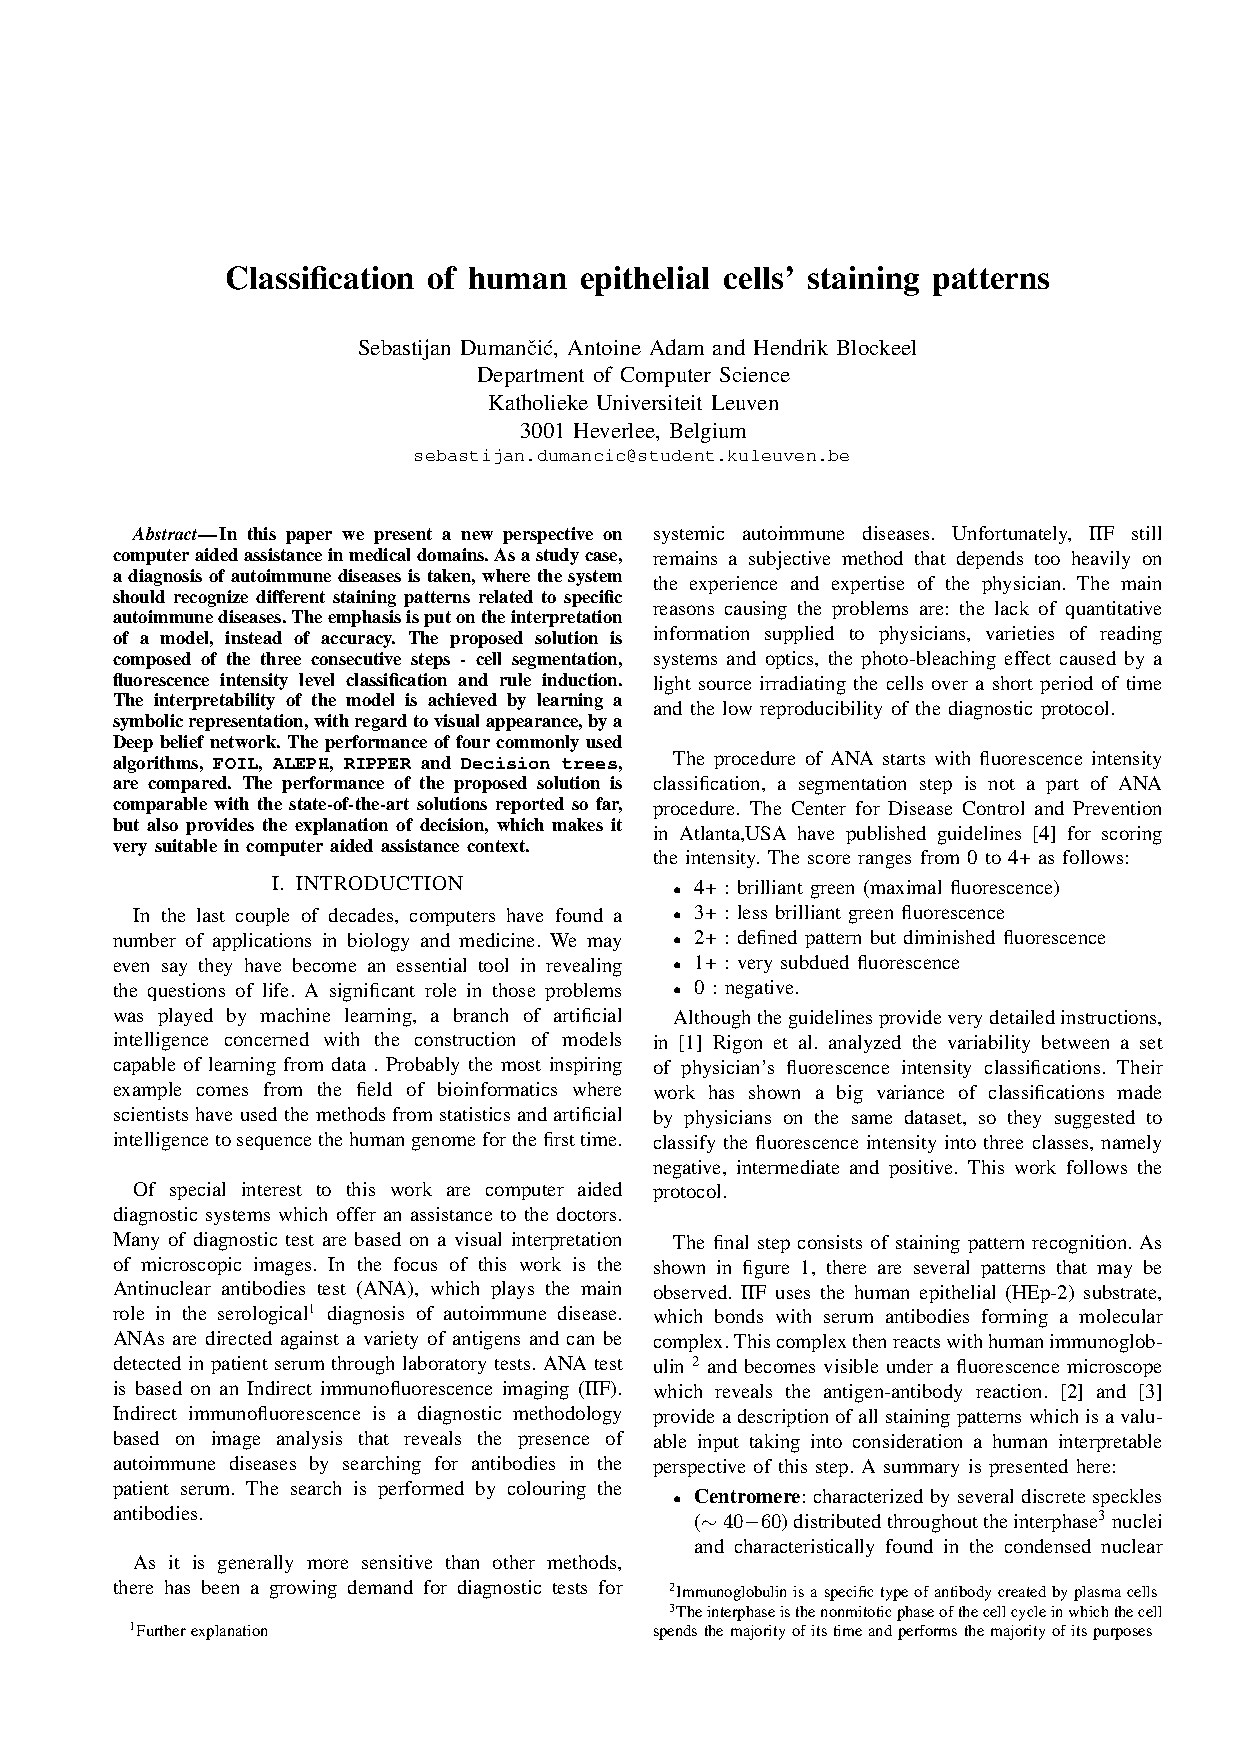
\includepdf[pages={1,2,3,4,5,6}]{../MasterThesis_paper/ieeeconf/paper.pdf}
% Chapter Template

\chapter{Induced rules} % Main chapter title

\label{AppendixB} % Change X to a consecutive number; for referencing this chapter elsewhere, use \ref{ChapterX}


In this appendix, the distributions of symbolic features are analyzed. The histogram of values for each symbolic features is plotted with regard to class.


%----------------------------------------------------------------------------------------
%	FEATURES
%----------------------------------------------------------------------------------------

\begin{figure}
	\caption{Rules induced by RIPPER }
	\label{fig:RulesRIPPER}
	\small
	\centering
	
		\begin{algorithmic}[1]
			\State \texttt{IF} number\_of\_obj = \textit{lots} 
			\Statex \texttt{THEN} \textit{centromere}
			\State \texttt{IF} mitotic\_cells = \textit{bright\_middle} 
			\Statex \texttt{THEN} \textit{homogeneos}
			\State \texttt{IF} organelle\_type = \textit{bright\_on\_dark} 
			\Statex \texttt{THEN} \textit{nucleolar}
			\State \texttt{IF} texture = \textit{rough} 
			\Statex \texttt{THEN} \textit{coarse speckled}
			\State \texttt{IF} shape = \textit{circular}  \texttt{AND} number\_of\_obj = \textit{few}
			\Statex \texttt{THEN} \textit{fine speckled}
			\State \texttt{IF} shape = \textit{irregular} 
			\Statex \texttt{THEN} \textit{cytoplasmatic}
			\State \texttt{IF} mitotic\_cells = \textit{dark spot} \texttt{AND} organelle\_type = \textit{neutral} 
			\Statex \texttt{THEN} \textit{fine speckled}
			\State \texttt{IF} intensity = \textit{intermediate} \texttt{AND} mitotic\_cells = \textit{neutral} 
			\Statex \texttt{THEN} \textit{nucleolar}
			\State \texttt{IF} mitotic\_cells = \textit{neutral} \texttt{AND} speckled = \textit{homogeneous} 
			\Statex \texttt{THEN} \textit{fine speckled}
			\State \textbf{else} \textit{cytoplasmatic}
		\end{algorithmic}
	
\end{figure}


\begin{figure}
	\caption{Rules induced by Decision tree }
	\label{fig:RulesDT}
	\footnotesize
	\centering
	
		\begin{algorithmic}[1]
			\State \texttt{IF} mitotic\_cells = \textit{bright middle} \texttt{AND} number\_of\_obj = \textit{few}
			\Statex \texttt{THEN} \textit{homogeneous}
			
			\State \texttt{IF} mitotic\_cells = \textit{bright middle} \texttt{AND} number\_of\_obj = \textit{lots}
			\Statex \texttt{THEN} \textit{centromere}
			
			\State \texttt{IF} mitotic\_cells = \textit{bright middle} \texttt{AND} number\_of\_obj = \textit{none}
			\Statex \texttt{THEN} \textit{homogeneous}
			
			\State \texttt{IF} mitotic\_cells = \textit{bright middle sparkle}
			\Statex \texttt{THEN} \textit{centromere}
			
			\State \texttt{IF} mitotic\_cells = \textit{dark spot} \texttt{AND} texture = \textit{blob}
			\Statex \texttt{THEN} \textit{cytoplasmatic}
			
			\State \texttt{IF} mitotic\_cells = \textit{dark spot} \texttt{AND} texture = \textit{rough} \texttt{AND} organelle\_type = \textit{bright\_on\_dark}
			\Statex \texttt{THEN} \textit{coarse speckled}
			
			\State \texttt{IF} mitotic\_cells = \textit{dark spot} \texttt{AND} texture = \textit{rough} \texttt{AND} organelle\_type = \textit{dark\_on\_bright} \texttt{AND} speckles = \textit{homogeneous}
			\Statex \texttt{THEN} \textit{fine speckled}
			
			\State \texttt{IF} mitotic\_cells = \textit{dark spot} \texttt{AND} texture = \textit{rough} \texttt{AND} organelle\_type = \textit{dark\_on\_bright} \texttt{AND} speckles = \textit{speckled}
			\Statex \texttt{THEN} \textit{coarse speckled}
			
			\State \texttt{IF} mitotic\_cells = \textit{dark spot} \texttt{AND} texture = \textit{rough} \texttt{AND} organelle\_type = \textit{neutral} 
			\Statex \texttt{THEN} \textit{coarse speckled}
			
			\State \texttt{IF} mitotic\_cells = \textit{dark spot} \texttt{AND} texture = \textit{smooth} \texttt{AND} organelle\_type = \textit{bright\_on\_dark} \texttt{AND} intensity = \textit{intermediate} 
			\Statex \texttt{THEN} \textit{fine speckled}
			
			\State \texttt{IF} mitotic\_cells = \textit{dark spot} \texttt{AND} texture = \textit{smooth} \texttt{AND} organelle\_type = \textit{bright\_on\_dark} \texttt{AND} intensity = \textit{positive} 
			\Statex \texttt{THEN} \textit{nucleolar}
			
			\State \texttt{IF} mitotic\_cells = \textit{dark spot} \texttt{AND} texture = \textit{smooth} \texttt{AND} organelle\_type = \textit{dark\_on\_bright} \texttt{AND} number\_of\_obj = \textit{few} 
			\Statex \texttt{THEN} \textit{fine speckled}
			
			\State \texttt{IF} mitotic\_cells = \textit{dark spot} \texttt{AND} texture = \textit{smooth} \texttt{AND} organelle\_type = \textit{dark\_on\_bright} \texttt{AND} number\_of\_obj = \textit{lots} 
			\Statex \texttt{THEN} \textit{fine speckled}
			
			\State \texttt{IF} mitotic\_cells = \textit{dark spot} \texttt{AND} texture = \textit{smooth} \texttt{AND} organelle\_type = \textit{dark\_on\_bright} \texttt{AND} number\_of\_obj = \textit{none} 
			\Statex \texttt{THEN} \textit{cytoplasmatic}
			
			\State \texttt{IF} mitotic\_cells = \textit{dark spot} \texttt{AND} texture = \textit{smooth} \texttt{AND} organelle\_type = \textit{neutral} 
			\Statex \texttt{THEN} \textit{fine speckled}
			
			\State \texttt{IF} mitotic\_cells = \textit{neutral} \texttt{AND} organelle\_type = \textit{bright\_on\_dark}
			\Statex \texttt{THEN} \textit{nucleolar}
			
			\State \texttt{IF} mitotic\_cells = \textit{neutral} \texttt{AND} organelle\_type = \textit{dark\_on\_bright} \texttt{AND} texture = \textit{rough} \texttt{AND} intensity = \textit{intermediate}
			\Statex \texttt{THEN} \textit{coarse speckled}
			
			\State \texttt{IF} mitotic\_cells = \textit{neutral} \texttt{AND} organelle\_type = \textit{dark\_on\_bright} \texttt{AND} texture = \textit{rough} \texttt{AND} intensity = \textit{positive}
			\Statex \texttt{THEN} \textit{fine speckled}
			
			\State \texttt{IF} mitotic\_cells = \textit{neutral} \texttt{AND} organelle\_type = \textit{dark\_on\_bright} \texttt{AND} texture = \textit{smooth}
			\Statex \texttt{THEN} \textit{fine speckled}
			
			\State \texttt{IF} mitotic\_cells = \textit{neutral} \texttt{AND} organelle\_type = \textit{neutral} \texttt{AND} number\_of\_obj = \textit{few}
			\Statex \texttt{THEN} \textit{nucleolar}
			
			\State \texttt{IF} mitotic\_cells = \textit{neutral} \texttt{AND} organelle\_type = \textit{neutral} \texttt{AND} number\_of\_obj = \textit{lots}
			\Statex \texttt{THEN} \textit{coarse speckled}
			
			\State \texttt{IF} mitotic\_cells = \textit{neutral} \texttt{AND} organelle\_type = \textit{neutral} \texttt{AND} number\_of\_obj = \textit{none} \texttt{AND} intensity = \textit{intermediate}
			\Statex \texttt{THEN} \textit{nucleolar}
			
			\State \texttt{IF} mitotic\_cells = \textit{neutral} \texttt{AND} organelle\_type = \textit{neutral} \texttt{AND} number\_of\_obj = \textit{none} \texttt{AND} intensity = \textit{positive}
			\Statex \texttt{THEN} \textit{fine speckled}
			
			\State \texttt{IF} mitotic\_cells = \textit{unknown} \texttt{AND} number\_of\_obj = \textit{few} 
			\Statex \texttt{THEN} \textit{nucleolar}
			
			\State \texttt{IF} mitotic\_cells = \textit{unknown} \texttt{AND} number\_of\_obj = \textit{none} 
			\Statex \texttt{THEN} \textit{cytoplasmatic}
			
		\end{algorithmic}
\end{figure}


\begin{figure}
	\caption{Rules induced by FOIL }
	\label{fig:RulesFOIL}
	\small
	\centering
	
		\begin{algorithmic}[1]
			\State \texttt{IF} organelle\_type = \textit{bright on dark} \texttt{AND} number\_of\_obj = \textit{lots} 
			\Statex \texttt{THEN} \textit{centromere}
			
			\State \texttt{IF} number\_of\_obj = \textit{lots} \texttt{AND} mitotic\_cells = \textit{bright middle}
			\Statex \texttt{THEN} \textit{centromere}
			
			\State \texttt{IF} intensity = \textit{intermediate} \texttt{AND} speckles = \textit{speckled} \texttt{AND} texture = \textit{rough}
			\Statex \texttt{THEN} \textit{coarse speckled}
			
			\State \texttt{IF} texture = \textit{rough} \texttt{AND} organelle\_type = \textit{neutral} \texttt{AND} mitotc\_cells = \textit{dark spot}
			\Statex \texttt{THEN} \textit{coarse speckled}
			
			\State \texttt{IF} intensity = \textit{positive} \texttt{AND} texture = \textit{rough} \texttt{AND} organelle\_type = \textit{dark on bright} \texttt{AND} number\_of\_obj = \textit{few} \texttt{AND} mitotic\_cells = \textit{dark spot}
			\Statex \texttt{THEN} \textit{coarse speckled}
			
			\State \texttt{IF} shape = \textit{irregular}
			\Statex \texttt{THEN} \textit{cytoplasmatic}
			
			\State \texttt{IF} texture = \textit{blob}
			\Statex \texttt{THEN} \textit{cytoplasmatic}
			
		\end{algorithmic}
	
\end{figure}
% ... and so on until
%\include{app-n}

\backmatter
% The bibliography comes after the appendices.
% You can replace the standard "abbrv" bibliography style by another one.
\bibliographystyle{abbrv}
\bibliography{Bibliography}

\end{document}

%%% Local Variables: 
%%% mode: latex
%%% TeX-master: t
%%% End: 
